% \newpage

% \subsection{Research questions \note{missing}}
% \subsection{motivation}


% \subsubsection{Energy Efficiency in Software Engineering}
% % Move this to soa or remove it 

% In their paper~\cite{pereira_energy_2017}, the authors studied the impact of programming languages on energy, time, and memory by using the CLBG benchmark, where they executed ten different benchmarks\footnote{\url{https://salsa.debian.org/benchmarksgame-team/benchmarksgame}} across 27 well-known programming languages~\cite{noauthor_pypl_2018}.

% The work of these authors was an extension of a research initiated by the work of \citeauthor{couto2017towards}~\cite{couto2017towards} to measure the impact of programming languages choice in real-life applications instead of micro-benchmarks.
% Irene~\emph{et~al.}~\cite{manotas_investigating_2013} Iren investigated the impact of web servers on energy when handling web applications.

% They analyzed seven applications executed across four servers in 38 different scenarios.
% The authors showed that the energy dramatically depends on the web server, but the impact of the application may also influence the energy behavior of the server.
% In their approach, they measured the energy consumption during the integration tests. At the same time, we are interested in simulating more realistic workloads and isolating the energy consumption of the server from the client's.

% Other works have been achieved on measuring the client applications' energy consumption; for example, ~\citeauthor{philippot_characterization_2014} concluded that there is a variation among the different websites and the impact of the browser on this energy consumption~\cite{philippot_characterization_2014}.

% % As we saw in the previous chapter, one of the most important things about a benchmark is how well it \textsc{reflects} the production environment.
% Therefore, we extend our study to cover real-world use cases, including two case studies reported in the following sections.

% TODO : incomplete and need rephrasing 

After studying the impact of the programming languages on energy consumption while handling the RPC requests, we found that the programing language and the web framework significantly impact energy consumption. Therefore, we want to delve deeper into this way.
This section will study not only the impact of programming languages but also the web frameworks on the energy consumption of the server.
Many studies have been conducted to compare the performance of web frameworks.
One can cite \cite{gajewski_analysis_2019} who compared two of the most famous Java frameworks---Play and Spring---or the work of \cite{benmoussa_new_2019} who compared different PHP frameworks using six criteria: intrinsic durability, industrialized solution, technical adaptability, strategy, technical architecture, and speed.
In our context, we push a $7^{th}$ criterion that impacts the economic outcome of the project.

We study the impact of web framework stacks on energy consumption. To do so, we implement a simple web application using the most popular web frameworks and compare their performance, latency, and energy consumption.  We leverage the \textsc{TechEmpower} \emph{Web Framework Benchmarks} to incorporate server-side energy measurements obtained from a software-defined power meter, named \textsc{PowerAPI}~\cite{fieni2020smartwatts}.
These measurements are then analyzed in depth to understand the critical criteria that can impact the power consumption of web frameworks and derive guidelines for supporting developers in picking the most energy-efficient web frameworks according to their requirements.

\subsection{Experimental Protocol}

\begin{figure}[!hbt]
    \centering
    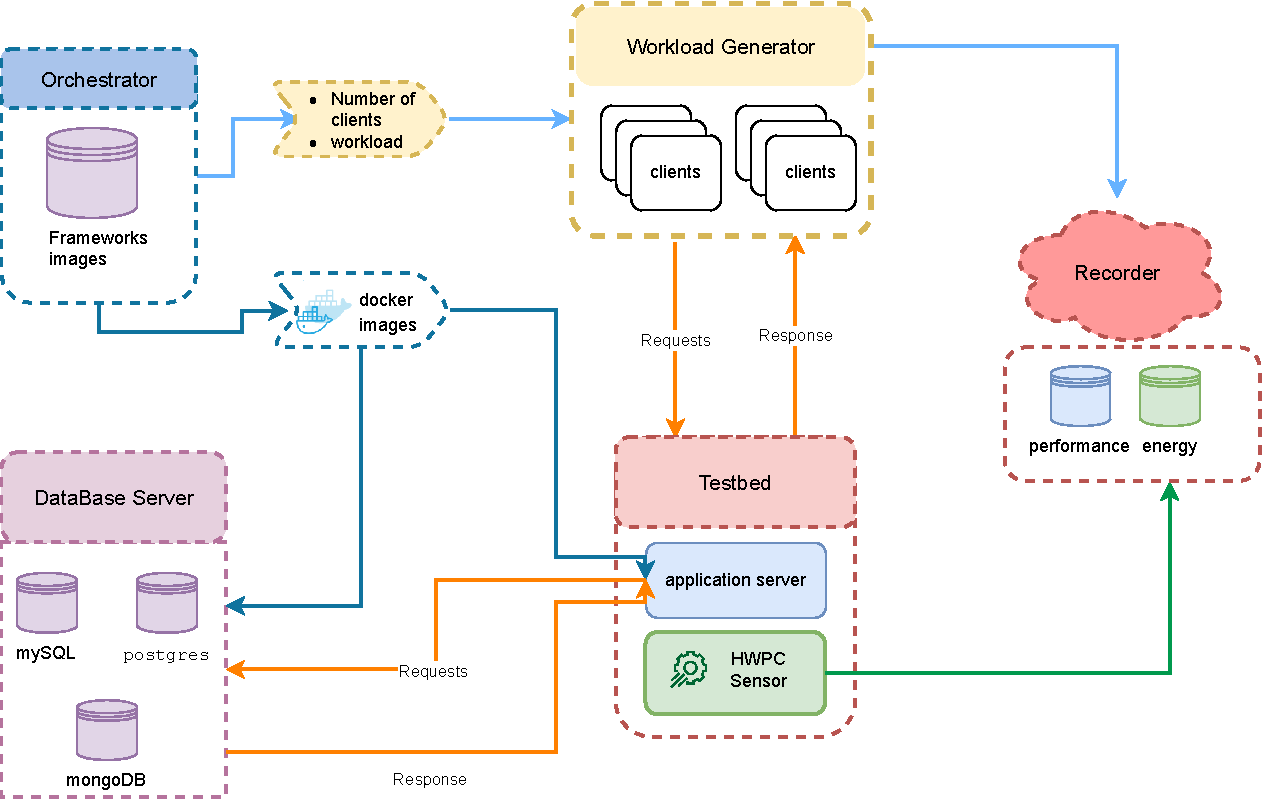
\includegraphics[width=.8\columnwidth]{imgs/architecture}
    \caption[Architecture]{Architecture of the experiments.}
    \label{fig:architecture}
\end{figure}

This section describes the environment we used during the experiments. Using the framework presented in \cref*{chapter:benchmarking}, we prepared a framework to measure the energy consumption of the web frameworks. The architecture of the experiments is presented in \cref{fig:architecture}.
As one can see, the system is composed of five key components:

\begin{itemize}
    \item \textsf{Orchestrator} is responsible for creating Docker images for each server, starting the server, and launching the benchmarks that the client should run,
    \item \textsf{web server}, or the \emph{system-under-test} (SUT), It is the server that we want to measure its energy consumption. The server is encapsulated in a Docker container to ease the deployment of the machine and ensure the reproducibility of the experiments,
    \item \textsf{database server} offers the database that all the frameworks will use during the benchmarks. It is separated from the application server to avoid the impact of the database on the energy consumption of the server,
    \item \textsf{client machine} It is responsible for stressing the web server using the scenarios provided by the orchestrator. To avoid the bottleneck on the client's side, we use \texttt{WRK}\footnote{\url{https://github.com/wg/wrk}}, a modern HTTP benchmarking tool,  capable of creating a large load, thanks to its multithreaded design and scalable event notification technologies such Epoll~\footnote{\url{https://man7.org/linux/man-pages/man7/epoll.7.html}} and Kqueue~\footnote{\url{https://man.openbsd.org/kqueue.2}}.
    \item \textsf{recorder} collects the power measurements from the SUT and the critical performance metrics collected by the clients, so later can be used for our empirical analysis.
\end{itemize}

Each component runs on a different machine to limit the outside impact on the server and the client. Such as the overhead of the database, creating and launching the servers, and storing the records of the experiments.
Moreover, all the machines belong to the same cluster to avoid network overhead.

% We will detail each component of the experiment and the tools we used to perform them.

% First, we start with the measurement context, which will cover the hardware and software components of the experiment.

\subsubsection*{Measurement Context}
This part describes the hardware and software components of the experiment.
\paragraph*{Hardware Settings}
All the tests have been executed in machines from the cluster \textsf{chetemi}~\footnote{\url{https://www.grid5000.fr/w/Hardware}} of the grid5000~\ref{cappello2010grid5000} platform.
This cluster comprises 15 machines with 2 Intel Xeon E5-2630 v4 processors, 256 GB of RAM,  600 GB HDD + 300 GB HDD hard disk.
For our experiment, we consider using four machines from this cluster, one for the orchestrator, one for the database server, one for the client, and one for the web server. As for the recorder part , the measures will be stored in a MongoDB Database that runs on a separate virtual machine.
\paragraph*{Software Settings}
Except for the recorder, all machines run a minimal version of Debian\,9 (4.9.0 kernel version), which enforces the core processes required for our experiment. Equipped with Docker, we can quickly deploy the web and database servers in a container.
\subsubsection{Measurement Context}
This experiment aims to highlight the energy impact of the technology stack used to develop web applications once in production.
To do so, we will use a web application composed of several URLs; each one will be used to simulate a test scenario. Therefore the clients will be agnostic to the technology stack used by the server.
Moreover, spilling the database on a remote server simulates a real-world scenario where the database is not hosted on the same machine as the web application. It allows us to isolate the energy consumption of the server, on the other hand.

\paragraph{Candidate Frameworks}
\begin{table*}
    \raggedright
    \caption{the number of framework passed per test }
    \label{table:frameworks_count}
    \begin{tabular}{l|c|c|c|c|c|c|c}
        \toprule
        Language    & Bb  & Query & Update & Plaintext & Fortune & Json & Total \\
        \midrule
        c           & 1   & 1     & 1      & 6         & 1       & 5    & 15    \\
        c\#         & 21  & 20    & 14     & 12        & 14      & 17   & 98    \\
        c++         & 27  & 16    & 14     & 20        & 13      & 25   & 115   \\
        cfml        & 2   & 1     & 1      & 1         & 1       & 2    & 8     \\
        clojure     & 8   & 8     & 5      & 6         & 7       & 8    & 42    \\
        common lisp & 2   & /     & /      & /         & /       & 2    & 4     \\
        crystal     & 3   & 1     & /      & 2         & /       & 2    & 8     \\
        d           & 3   & 2     & 1      & 2         & 1       & 3    & 12    \\
        dart        & /   & /     & /      & 2         & /       & 2    & 4     \\
        elixir      & 1   & 1     & /      & /         & /       & 1    & 3     \\
        erlang      & 3   & 2     & /      & 3         & 1       & 3    & 12    \\
        f\#         & /   & /     & /      & 4         & 2       & 8    & 14    \\
        go          & 19  & 18    & 16     & 15        & 15      & 19   & 102   \\
        groovy      & 1   & /     & /      & 1         & /       & 2    & 4     \\
        haskell     & 1   & 1     & 1      & 2         & 1       & 2    & 8     \\
        java        & 20  & 20    & 18     & 26        & 21      & 26   & 131   \\
        javascript  & 19  & 19    & 16     & 14        & 17      & 14   & 99    \\
        julia       & /   & /     & /      & 1         & /       & 1    & 2     \\
        kotlin      & 10  & 9     & 6      & 5         & 5       & 10   & 45    \\
        lua         & 1   & 1     & /      & 1         & 1       & 2    & 6     \\
        nim         & /   & /     & /      & 2         & /       & 3    & 5     \\
        ocaml       & 4   & 4     & 3      & 1         & 2       & 5    & 19    \\
        perl        & 2   & /     & /      & 1         & /       & 2    & 5     \\
        php         & 22  & 18    & 15     & 10        & 12      & 14   & 91    \\
        prolog      & /   & /     & /      & 1         & /       & 1    & 2     \\
        python      & 31  & 21    & 15     & 17        & 16      & 30   & 130   \\
        racket      & 1   & /     & /      & /         & /       & /    & 1     \\
        ruby        & 23  & 15    & 11     & 8         & 12      & 19   & 88    \\
        rust        & 8   & 7     & 6      & 9         & 8       & 10   & 48    \\
        scala       & 7   & 6     & 3      & 8         & 5       & 11   & 40    \\
        swift       & 2   & 2     & /      & 2         & /       & 2    & 8     \\
        typescript  & 4   & 2     & 2      & 3         & 2       & 6    & 19    \\
        v           & /   & /     & /      & 1         & /       & 1    & 2     \\
        vala        & /   & /     & /      & 1         & /       & 2    & 3     \\
        vb          & 2   & 2     & 2      & 1         & 2       & 1    & 10    \\
        \midrule
        total       & 248 & 197   & 150    & 188       & 159     & 261  & 1203  \\
        \bottomrule
    \end{tabular}

\end{table*}
Overall, we selected 210 web frameworks to be evaluated in this study.
Each framework may have several configurations depending on the database, alternative interpreters, and so on.
Table~\ref{table:frameworks_count} highlights the number of frameworks used in the experiment per benchmark category.
As we see in this table, some of the frameworks worked on certain conditions, while they failed on other benchmarks, such as Nickel (based on Rust).
While it might be one of the most energy-efficient Rust frameworks, Nickel does not work with databases.
Therefore, it cannot be used for any situation, but if a (stateless) web application does not interact with a database, it might be the best choice.
Many reasons are behind the observed failures; there was no implementation, some errors were raised when handling the request, or simply the framework does not support such a feature.

\subsubsection{Input Workload}

In order to compare the energy consumption and performance efficiency of various frameworks, each framework is used to implement the same web application---\emph{i.e.}, replying to the same HTTP endpoints and requesting the same database. Then, we run the same sequence for all the SUT:
\begin{enumerate}
    \item lunch the web application,
    \item wait for the 20s for the warmup,
    \item measure the average power when the application is in an idle state,
    \item using multiple clients, we send the same request concurrently during the 20s,
    \item increase the number of parallel requests,
    \item measure the energy during this execution,
    \item changes the request type,
    \item repeat from the $3^{rd}$ step.
\end{enumerate}

The following sections describe each type of experiment and its purpose by giving some examples of the expected responses.

\paragraph{Test Scenarios}
We have seven categories of benchmarks:
\paragraph{Idle}
In this benchmark, we measure the web framework's idle energy consumption; this reflects an application's average energy consumption during periods without connections, for example, a company website beyond working hours or an online shop at night.

\paragraph{Single Query}
Each request in this scenario is handled by retrieving a single row from a simple database table.
This row is then serialized and returned to the client as a JSON response.
In a web application, this is the most common sort of request.
We employ a variable number of clients to measure the energy usage of the web framework when it is under load for this benchmark.



\paragraph{Multiple Queries}
This benchmark aims to observe the behavior of a web framework when it processes multiple entries from the database.
Therefore, as a result, each request is handled by retrieving numerous rows from a simple database table,then serializing them as a JSON response.
This benchmark's purpose is to observe a web framework's behavior while increasing the number of rows.
In this case, we will use 512 clients.
% and alter the
%The benchmark is run multiple times: benchmarking 1, 5, 10, 15, and 20 queries per request. All benchmarks are run at 512 concurrency.
% To evaluate the performance of a framework when the data is already cashed  each request is processed by fetching multiple cached objects from an in-memory database and serializing these objects as a JSON response.
%  The benchmark is run multiple times: benchmarking 1, 5, 10, 15, and 20 cached object fetches per request. All benchmarks are run at 512 concurrency. Conceptually, this is similar to the multiple-queries benchmark except the fact that it uses a caching layer.

\paragraph{Fortunes}
The purpose of this scenario is to study the behavior of a web framework when it processes a request that requires a database query and a template rendering.
To do so, we ask the framework to retrieve all the rows from our database (in our case, 12 rows) and then send the response as a generated HTML page.
The stress level varies according to the number of parallel clients.

\paragraph{Update Queries}
This scenario puts the database \texttt{write} to the test.
Each request is handled by retrieving numerous rows from a simple database table, turning the rows into in-memory objects, altering one attribute of each object in memory, individually updating each related row in the database, and serializing the list of objects as a JSON response.
Like the previous benchmarks, we will use 512 clients and vary the number of rows retrieved from the database according to the stress level.

\paragraph{Plain Text}
In this scenario, the server responds with a simple message, \texttt{"Hello, World!"} in plain text.
Thanks to the small message size, we can enable the HTTP pipelining on the client side, which leads to greater client-side concurrency levels.


\paragraph{JSON Serialization}
In this scenario, the server returns a new instance of a JSON object with the following structure. \texttt{\{"message": "Hello, World!"\}}.

\paragraph{Recap}

Table~\ref{frameworks:stress-levels} recaps different stress levels of each scenario above. Whenever the stress level is based on the size request, we use the same size of clients (512); otherwise, we use the number of clients as the stress level.

\begin{table*}[bth]
    \raggedright
    \caption{Stress levels for each scenario.}
    \label{frameworks:stress-levels}
    \resizebox{\textwidth}{!}{
        \begin{tabular}{l|l|c|c|c|c|c|c|c|}
            \toprule
            \textbf{Scenario}  & \textbf{type of stress}                  & \textbf{level 1} & \textbf{level 2} & \textbf{level 3} & \textbf{level 4} & \textbf{level 5} & \textbf{level 6} & \textbf{level 7} \\
            \midrule
            Single Query       & Number of parallel clients               & 16               & 32               & 64               & 128              & 256              & 512              & /                \\
            Multiple Queries   & Number of rows to read from the database & 1                & 5                & 10               & 15               & 20               & 30               & 50               \\
            Update Queries     & Number of rows to update in the database & 1                & 5                & 10               & 15               & 20               & 30               & 50               \\
            Fortunes           & Number of parallel clients               & 16               & 32               & 64               & 128              & 256              & 512              & /                \\
            JSON Serialization & Number of parallel clients               & 16               & 32               & 64               & 128              & 256              & 512              & /                \\
            Plain Text         & Number of parallel clients               & 256              & 1024             & 4096             & 16384            & 32384            & /                & /                \\
            \bottomrule
        \end{tabular}
    }
\end{table*}

To include additional scenarios, one might implement a Python class that handles the metadata of the workload, such as the query route, the query parameters, and the expected results.

\subsubsection{Key Performance Metrics}
We focus on comparing the energy behavior of different frameworks in multiple scenarios.
To measure the energy consumption of those frameworks, we launch each one for a fixed duration, and then all the clients send multiple requests simultaneously.
We compute the number of satisfied responses, which reflects the performance of the framework, the average latency, and the global energy consumed during the whole period, to deduce the energy cost of each request.

\paragraph{Runtime Measurements}
\begin{itemize}
    \item energy measurement :
          We use PowerAPI~\cite{bourdon:hal-00772454}, a software power meter, to gather the power consumption of the SUT after we project the timestamps of each experiment phase to calculate the energy consumption of the framework during this phase.
          Energy is an integral of power over time, so we use a numerical approach to isolate the energy consumption.%~\ref{fig:trapezrule}.
          After this, we divide the calculated energy per the number of responses.
          % \begin{figure}[hbt]
          %     \centering
          \begin{equation}
              E = \int^a_b P(t)dt \simeq \sum^n_{k=1} \frac{P(t_k-1)+P(t_k)}{2}
          \end{equation}
          %     \caption{}
          %     \label{fig:trapezrule}
          % \end{figure}
          %   During this phase, we collce
          %   we have 4 metrics :
    \item Total cost of the energy during each period,
    \item Total number of requests,
    \item latency of the responses,
    \item Average energy cost per request.
\end{itemize}
\paragraph{Notes}
Due to technical problems, not all the web frameworks returned the tail latency (99\%). Therefore we substitute it with the average latency during this study.
However, for further details, the reader can always check the available values in our public repository.\footnote{\url{https://github.com/chakib-belgaid/}}


It has been proven in the work of \citeauthor{eddie_antonio_santos_how} that Docker does not impact energy consumption.
Thus, using containers and isolation avoids any noise of the operating system after executing one benchmark and contributes to the reproducibility of our results.

\paragraph{Bias Analysis}
We are aware of potential bias analysis regarding estimating the total energy cost, the interference of other system processes during the execution, and some external events.
Thus, we run experiments multiple times and compute the average values.

\subsubsection{Extension}
To follow the guidelines that we presented in Chapter~\ref{chapter:benchmarking}, we provide a GitHub repository\footnote{\url{https://github.com/chakib-belgaid/FrameworkBenchmarks}} where one can add extra \textbf{candidates} by creating a new project using the option \texttt{--new}.
Then, interested practitioners must fill out the template and provide the Docker image file.
Additionally, to configure the \textbf{workload} we provide the option \texttt{--concurrency-levels} and \texttt{--duration}.
The choice of the database is included in the Docker image.

\subsection{Results \& Findings}


, and all can be found in the online repository.\footnote{\url{https://github.com/chakib-belgaid/frameworks-benchmarks-results}}
Due to the extensive number of results (261 frameworks), we could not compare frameworks individually. Instead, we will aggregate our results based on the language family. However, in the end, we provide a dashboard that allows the reader to explore the results in more detail and compare several frameworks.
We will group the frameworks not by language but by family so that we will have five families:
\begin{itemize}
    \item \textbf{compiled languages}: Rust, Go, Haskell, C++, C, Vala, Nim, Swift, Prolog, V, Ocaml, Crystal, and D;
    \item \textbf{interpreted languages}: Javascript, Python, Lua, Php, Cfml, Racket, Ruby, Common lisp, Perl, Julia, Groovy, and Typescript;
    \item \textbf{JVM-based languages}: Java, Kotlin, Scala, and Clojure;
    \item \textbf{.Net-based languages}: C\#, F\# and VB;
    \item \textbf{Other VM-based languages}: Dart and Elixir and Erlang.
\end{itemize}
% In this section, we discuss these results to answer the following questions:
% \begin{itemize}
%     \item [\textsc{RQ}~1:] is there a dominating family language regarding performance, energy consumption, and latency?
%     \item [\textsc{RQ}~2:] which class of family language is performing well?
%     \item [\textsc{RQ}~3:] is there a correlation between energy consumption and latency?
%     \item [\textsc{RQ}~4:] is there an impact on the server when it comes to changing the database?
% \end{itemize}

\subsubsection{Overall Statistics}

To determine which web framework/stack is performing well, we need to establish some general idea about the average energy consumption and latency of the frameworks under study.
Instead of reporting the raw energy consumption of those frameworks, we will provide some green factors to determine which one is eco-friendly and which is greedy.
In this part, we will discuss the average behavior of the frameworks, highlight some trends, and eliminate the outliers.
A gentle reminder that being an outlier, in this case, does not mean that the web framework is not performing well; it means that the web framework is not performing well in the same way as the others within the context of this experiment.

First, we will perform a correlation test between the metrics to narrow the research space.

Because the Shapiro-Wilk~\cite{shapiro1968comparative} test yielded a $p$-value of 0.0 for all metrics, our data do not follow a normal distribution. Therefore, we use The non-parametric test known as Pearson correlation coefficient~\cite{zar2005spearman}

\begin{figure}[!h]
    \centering
    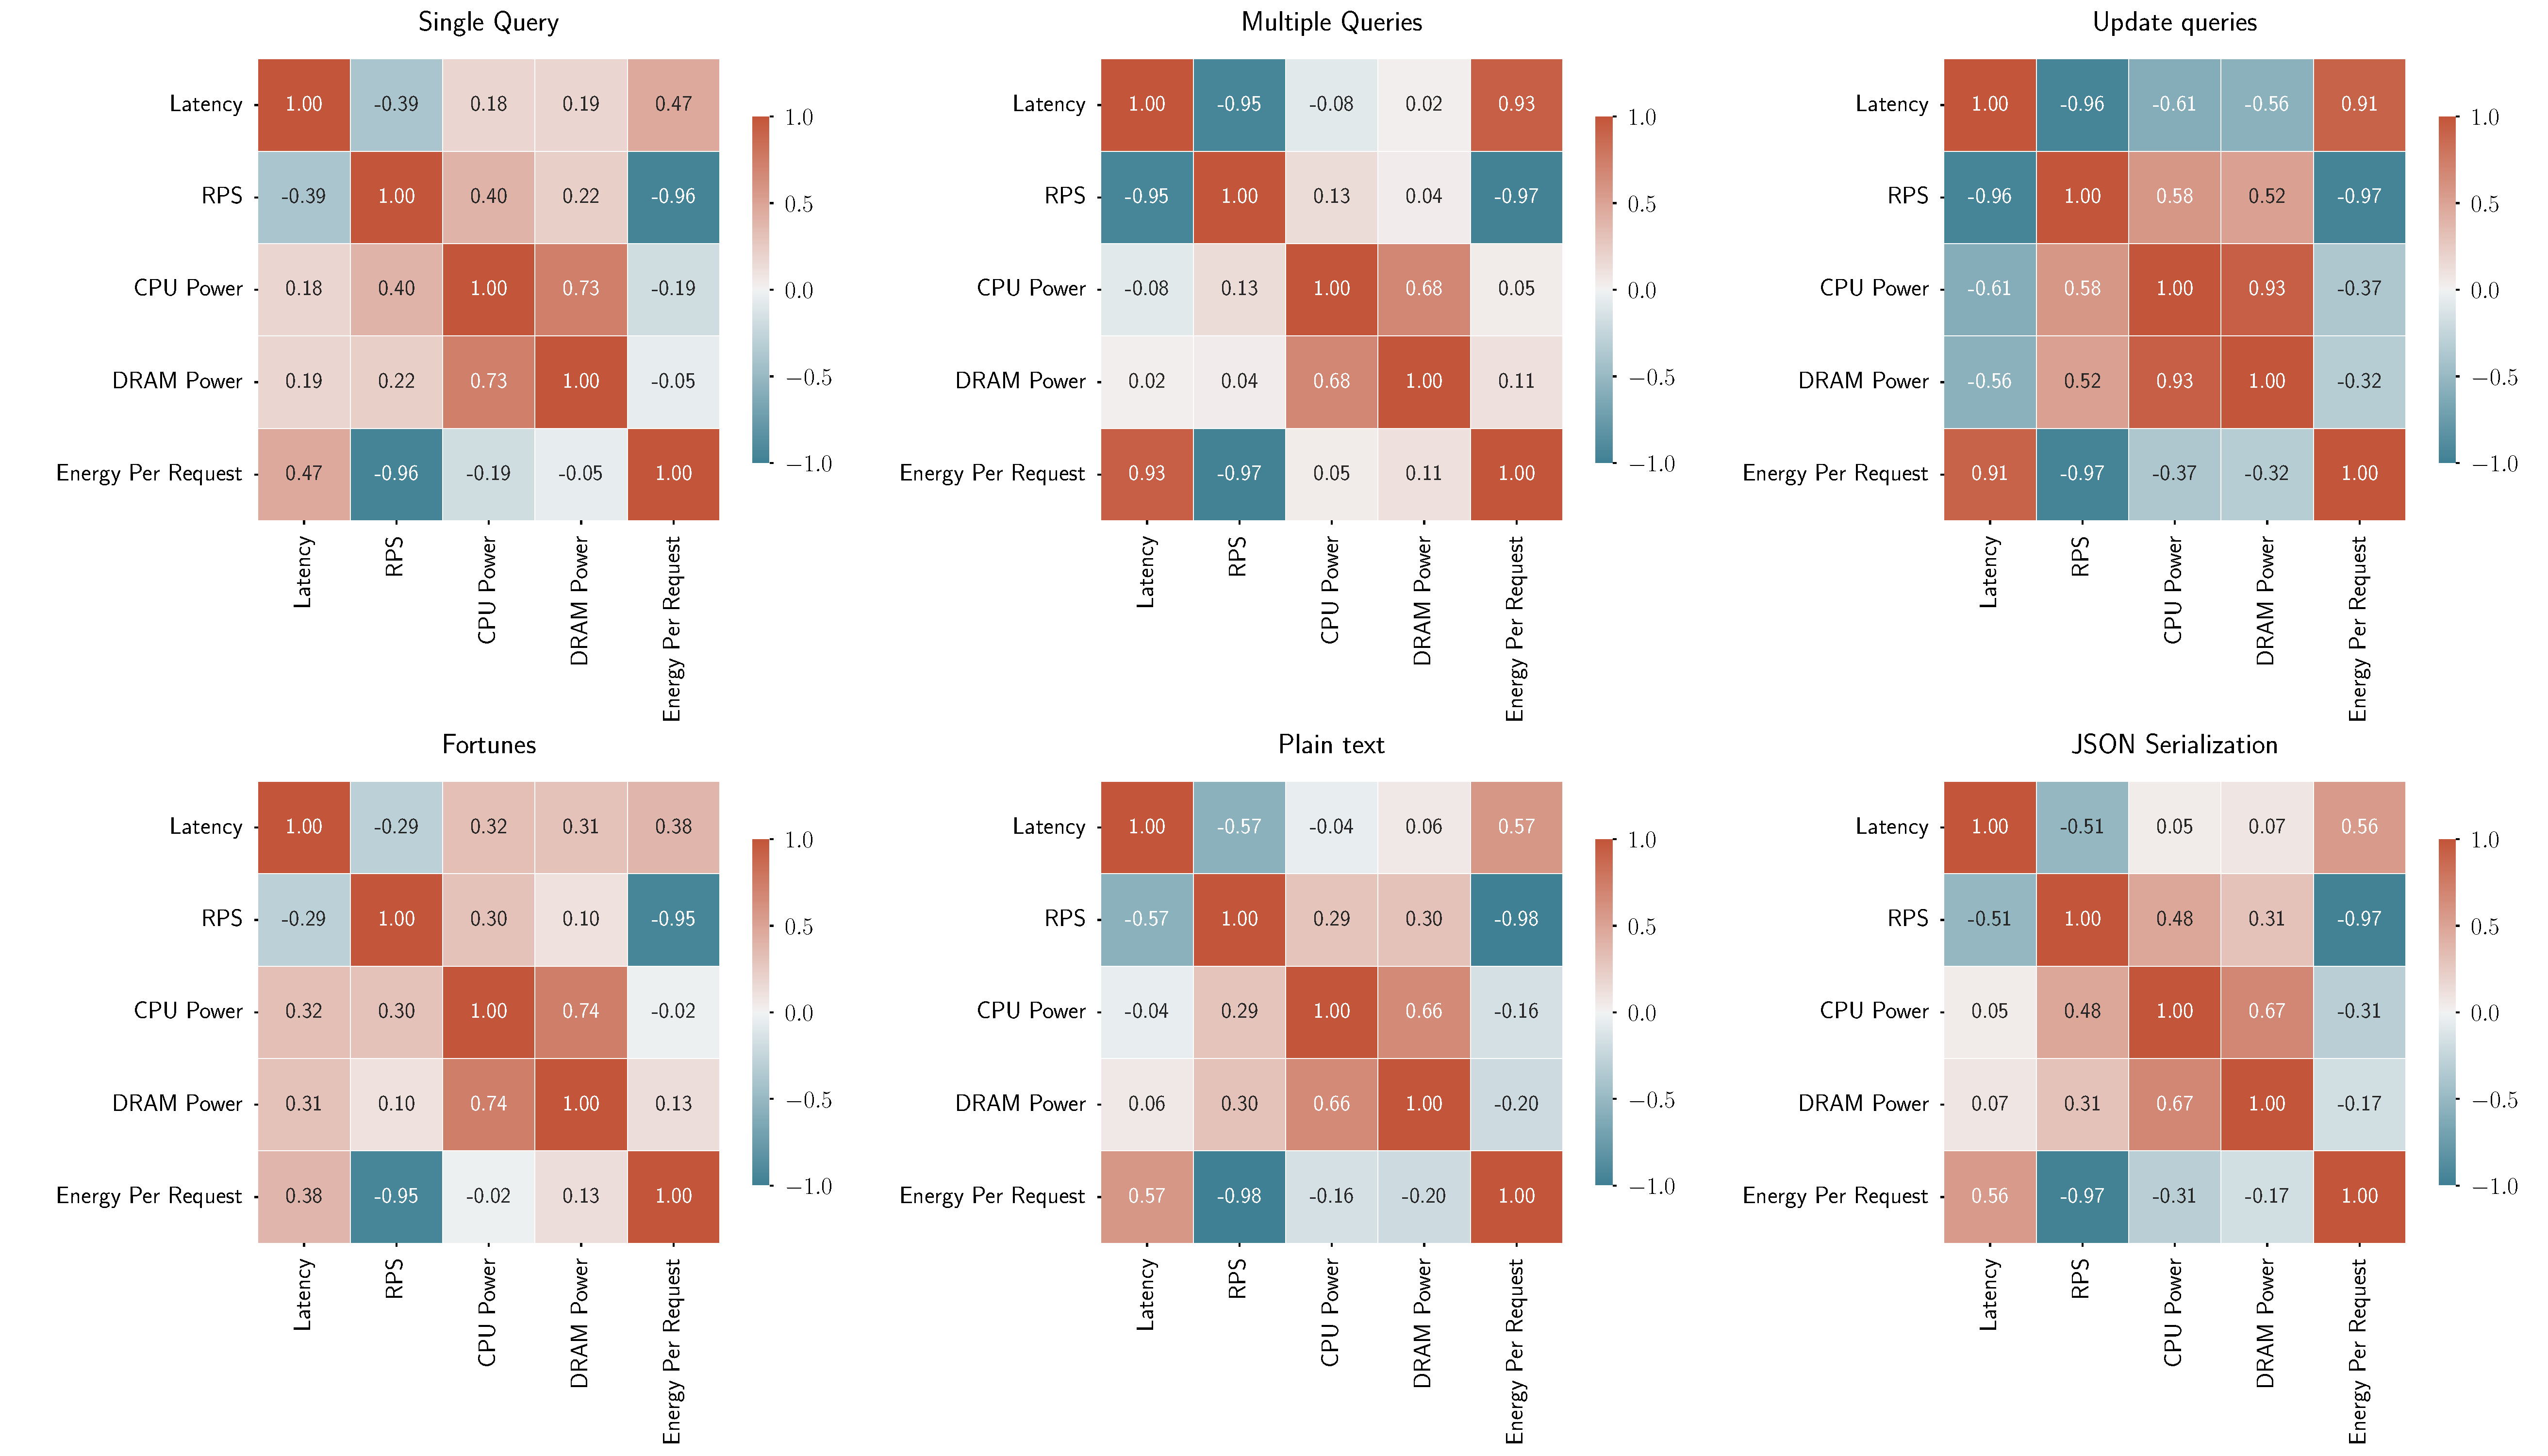
\includegraphics[width=\textwidth]{imgs/correlation_all}
    \caption{Spearman Rank Correlation between different metrics}
    \label{fig:correlation}
\end{figure}

Figure~\ref{fig:correlation} depicts the correlation between the metrics for the 6 scenarios.
The Pearson correlation coefficient quantifies the linear correlation between two variables, X and Y.
It ranges from -1 to +1, with 1 being total positive linear correlation, 0 representing no linear correlation, and -1 representing whole negative linear correlation.
The stronger the correlation, the closer the value is to 1 or -1.
The weaker the correlation, the closer the value is to zero.
The Pearson product-moment correlation coefficient is another name for the correlation coefficient.
This correlation coefficient is also known as the Pearson product-moment correlation coefficient.
One can notice that there is a strong correlation between the energy consumption of the CPU and the DRAM for most of the scenarios.
Moreover, the average energy consumption of DRAM is one-sixth of the CPU energy consumption.
Therefore, this study will focus more on CPU energy consumption.
For more insights about the DRAM consumption, we refer the reader to our GitHub repository.\footnote{\url{https://github.com/chakib-belgaid/frameworks-benchmarks-results}}

Another strong correlation is between the number of requests per second and the average cost of a single request.
This strong correlation happens because the cost of a single request is proportionate to the number of requests per second since the Average Power consumption remains constant after a certain threshold of clients; one should remember that this limit is different for each framework.

Unlike the \emph{multiple queries and update} queries, the single query scenario depicts a weak correlation between latency and the number of requests per second.
The reason behind such an anomaly is the fact that we summarized the data when we had multiple numbers of clients.
If we calculate the correlation when we have a fixed number of clients, like in the case of update queries (512 clients), one can notice a strong correlation. Figure~\ref{fig:scatter_db} demonstrates such a behavior. As one can notice, for each level, we observe a linear clustering.

\begin{figure}[!h]
    \centering
    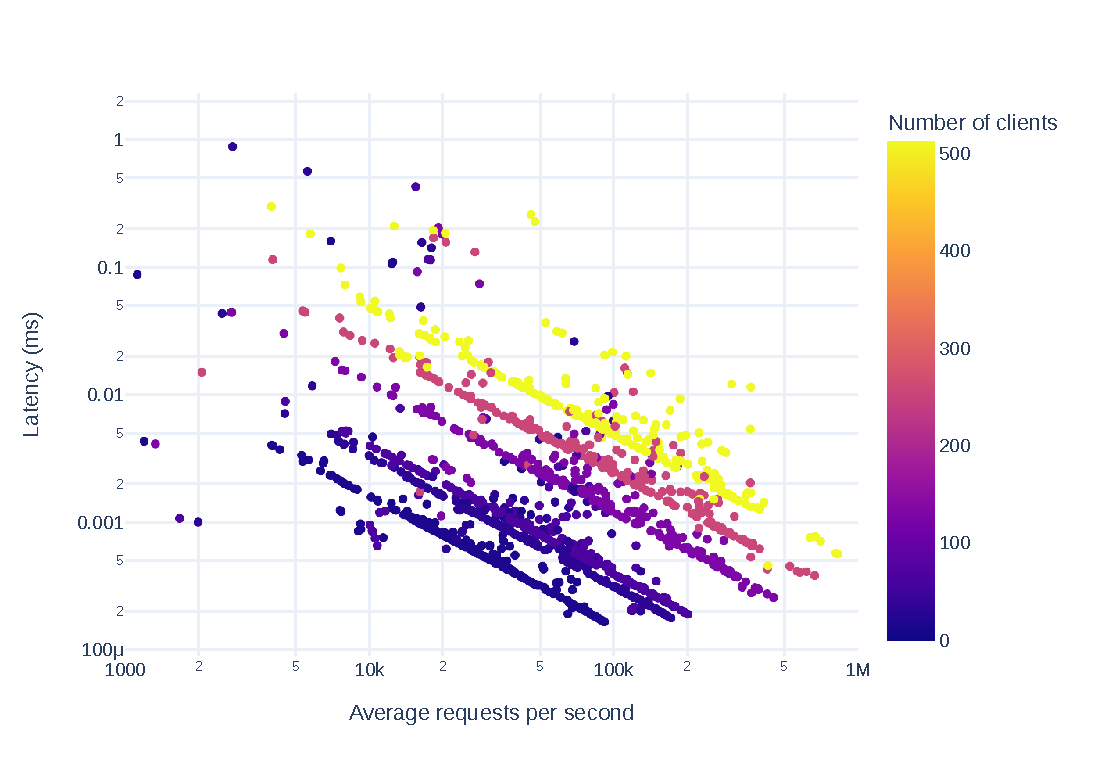
\includegraphics[width=.9\columnwidth ]{imgs/scatter_db_latency_rps}
    \caption{Correlation of latency and number of requests per second for a single query}
    \label{fig:scatter_db}
\end{figure}

Therefore, we can safely focus our analysis on two variables, \emph{number of requests per second} and \emph{average energy consumption}. The first one will indicate the performance of the solution. Meanwhile, the second one will measure how green a framework is.



%  THIS might be completely changed , i think we need to check the limits of the data base 

% inherently there is no correlation between the energy consumption of the CPU and the latency, which means that we can achieve both a low latency and low energy consumption simultaneously. 


\subsubsection{Scenario-based Analysis}
After establishing the general idea about the average behavior of the frameworks, we will now focus on the analysis of each scenario.

\paragraph{Idle behviour}
This part will treat average power behavior when the framework is in a rest mode.
Figure~\ref{fig:av_power_idle} presents, a density plot for each family.

\begin{figure}[!h]
    \centering
    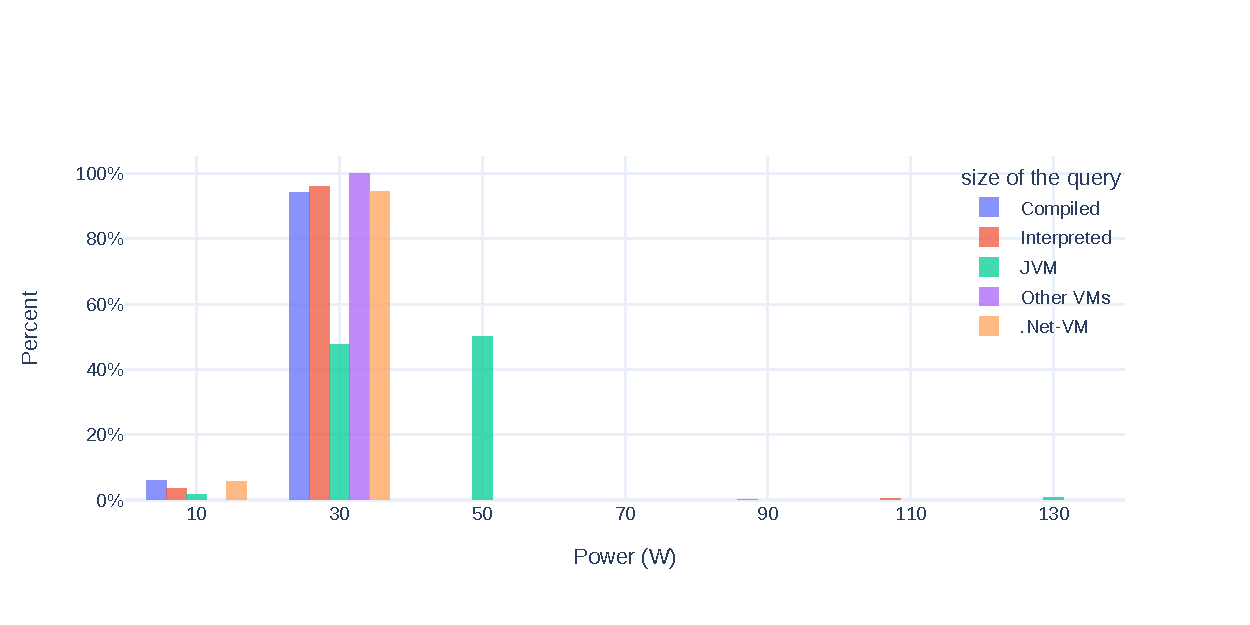
\includegraphics[width=1.0\columnwidth]{imgs/av_power_idle}
    \caption{Average power consumption for the idle scenario}
    \label{fig:av_power_idle}
\end{figure}

As one can notice at rest, most families consume between 20 and 40 Watts, and 6\% of the compiled language frameworks consume less than 15 Watts.
However, 50\% of Java solutions tend to consume around 50 Watts, which makes it the most greedy family.
If we look at each of the programming languages from Java separately in Figure~\ref{fig:av_power_java_idle}, we find that Java-based implementations tend to consume around 50 Watts. In contrast, Kotlin, Clojure, and Scala consume around 30 Watts, the same consumption as the other families.

\begin{figure}[!h]
    \centering
    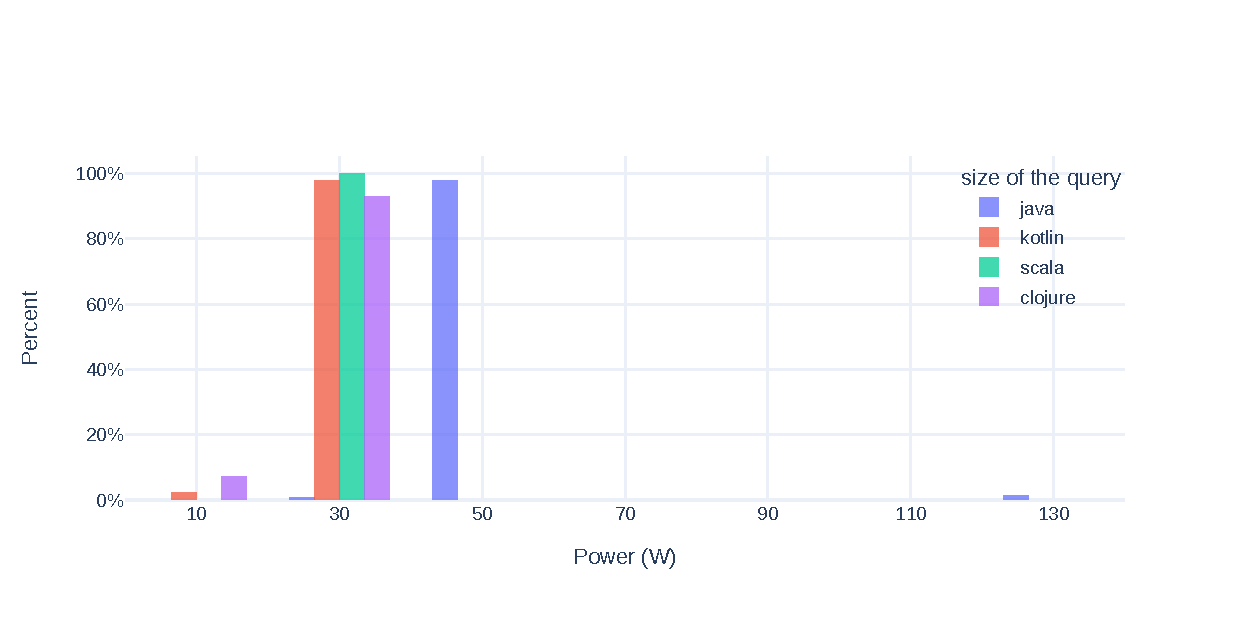
\includegraphics[width=1.0\columnwidth]{imgs/av_power_java_idle}
    \caption{Average power consumption for Java-based languages in the idle scenario case}
    \label{fig:av_power_java_idle}
\end{figure}

\paragraph{Single query}
As mentioned before, the purpose of this scenario is to benchmark the framework efficiency to handle a single entry.
We will start with an average power consumption histogram to determine the frameworks' general behavior.
Figure~\ref{fig:av_power_db} reports the density plot of average power consumptions for all the experiments depending on the number of concurrent clients.
As one can observe, there are three main states:
\begin{enumerate}
    \item \emph{relaxed state} where the number of clients is less than 16: most of the frameworks consume around 70 Watts;
    \item \emph{average state} where the number of clients is between 16 and 64: most of the frameworks consume around 100 Watts;
    \item Finally, the \emph{stress state} beyond 128 concurrent clients: most frameworks have a stable power consumption regardless of the number of clients. This increase in power consumption is due to the database server, which reached its maximum capacity.
\end{enumerate}

\begin{figure}[!h]
    \centering
    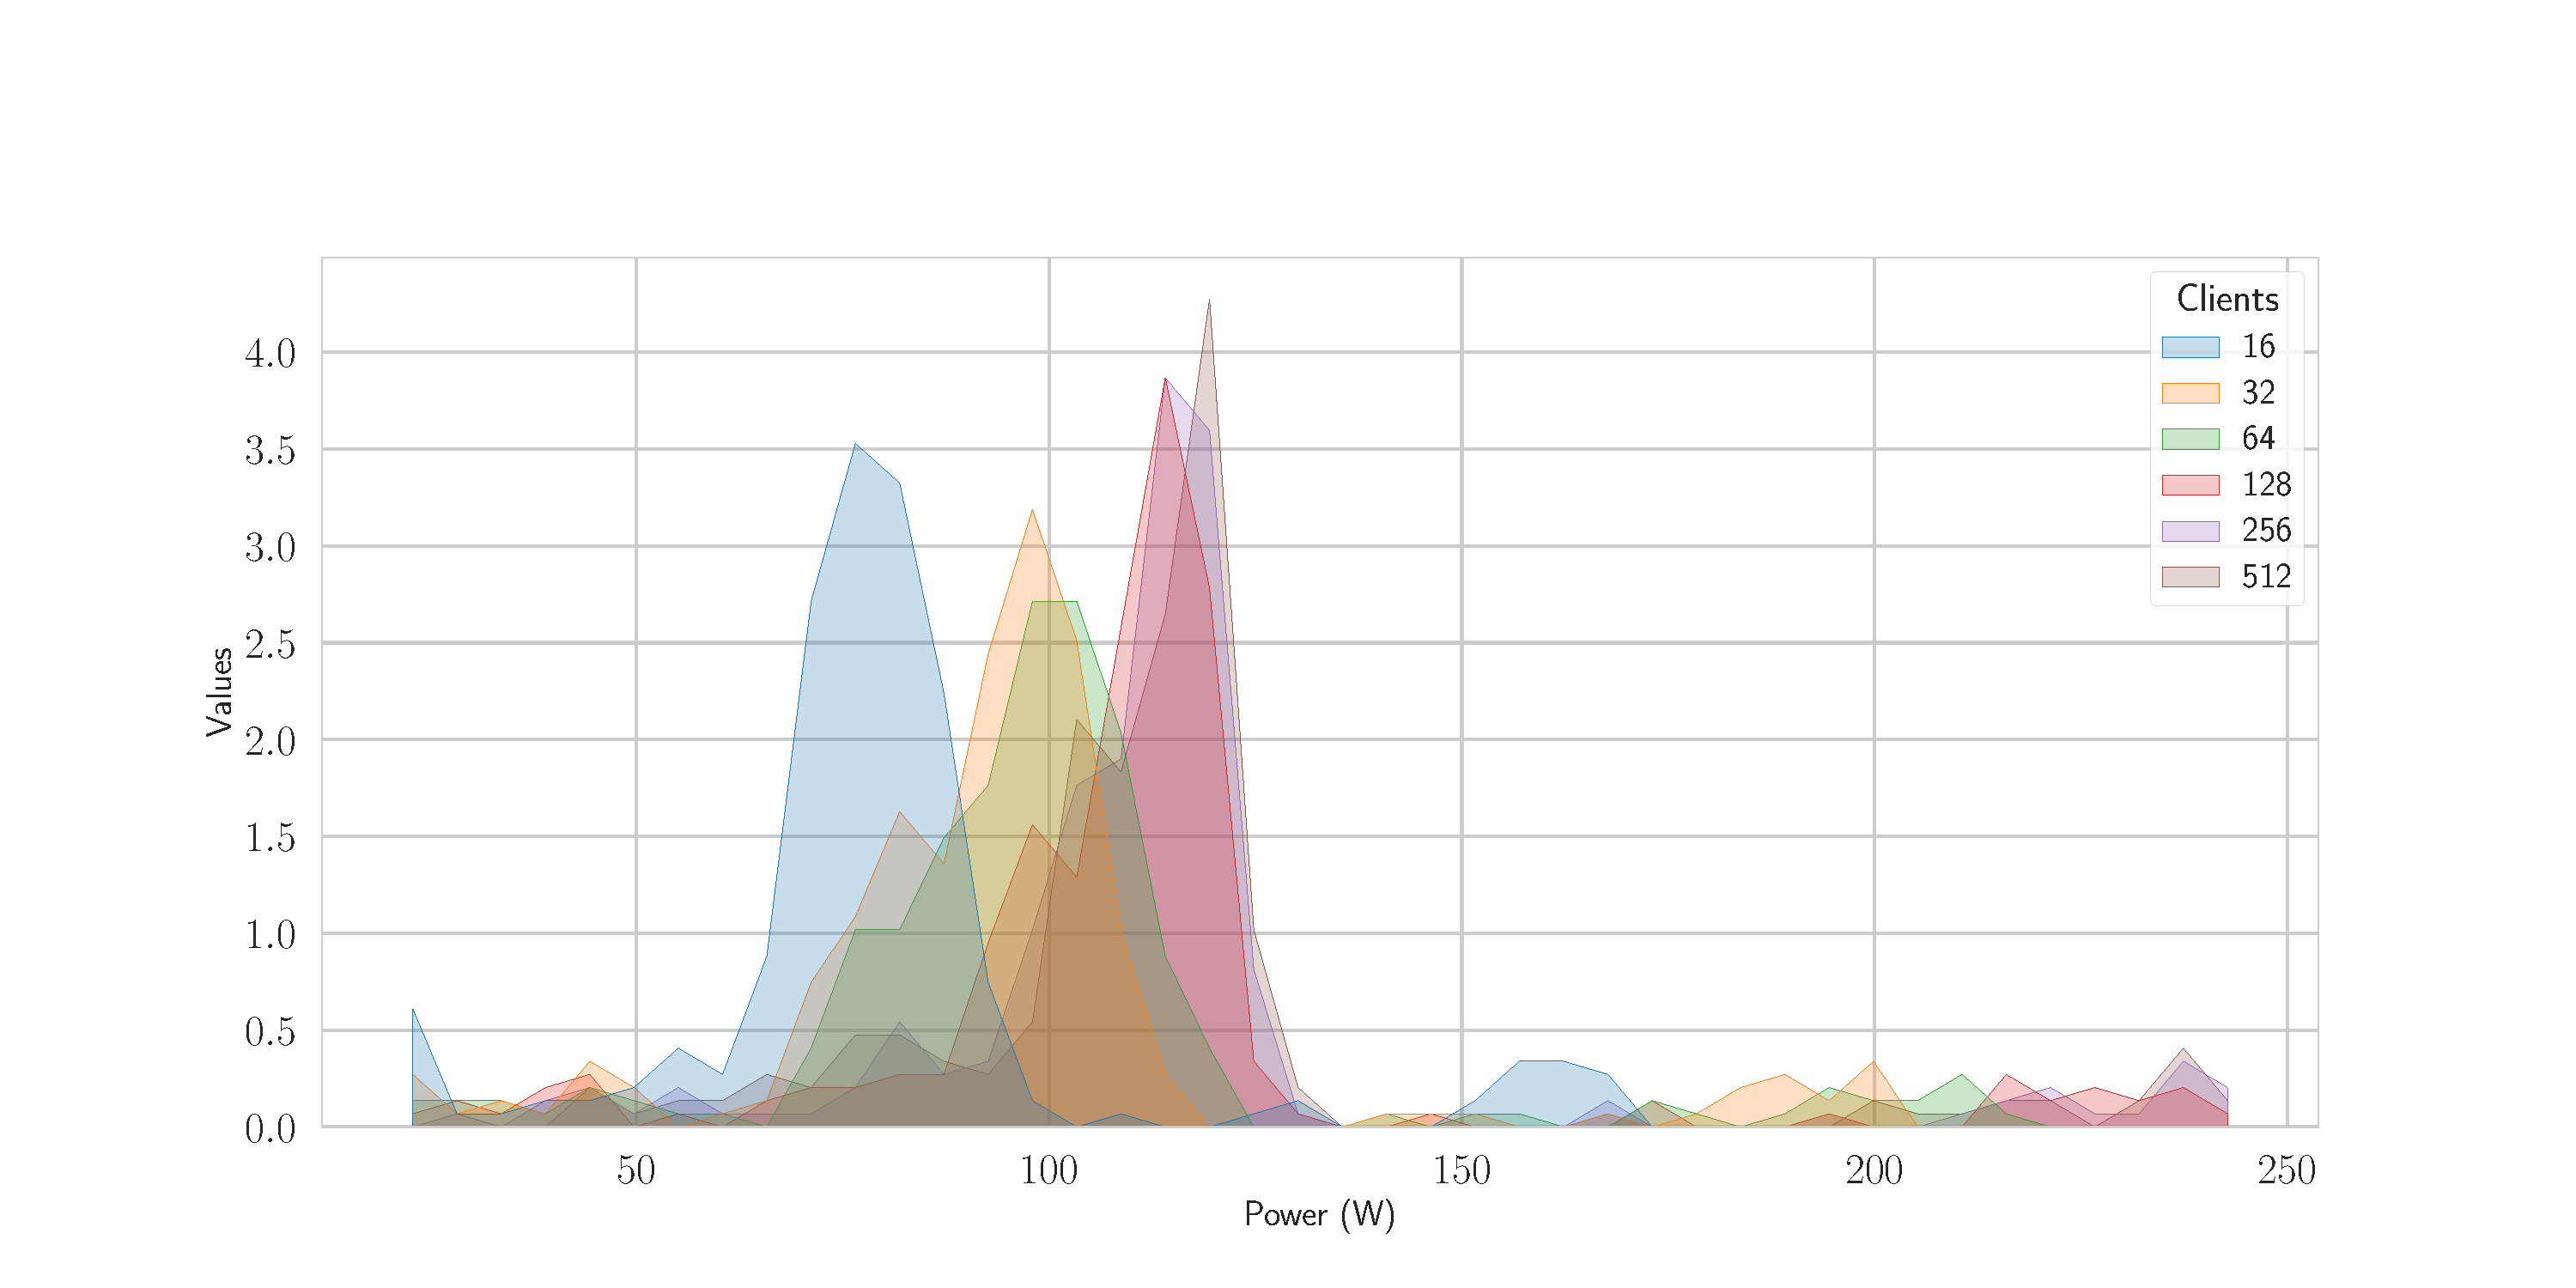
\includegraphics[width=\textwidth,height=\textheight,keepaspectratio]{imgs/histogram_av_power_cpu_db}
    \caption{Distribution of the average power consumption for \emph{single query} scenario }
    \label{fig:av_power_db}
\end{figure}

Now that we have seen the overall distribution of the power within the single query scenario.
We analyze each family separately.
In addition, we include the number of \emph{requests per second} (RPS) as a performance metric of interest.
In Figure~\ref{fig:power_requests_db}, each run is represented by a circle, and the size of the circle indicates the number of concurrent clients: The smaller the circle, the fewer clients.
On the one hand, one can notice that compiled languages are the most efficient in terms of performance, despite their average energy consumption.
Moreover, there is no significant change in the average power consumption when we increase the number of concurrent clients.
On the other hand, the JVM-based frameworks tend to consume the most energy while reporting the same performance as the .Net-based ones.
Finally, the interpreted languages lack performance while keeping low power, except for PHP, as it has one of the highest RPS with a half million RPS which got beaten only by C++ and Rust.

\begin{figure}[!h]
    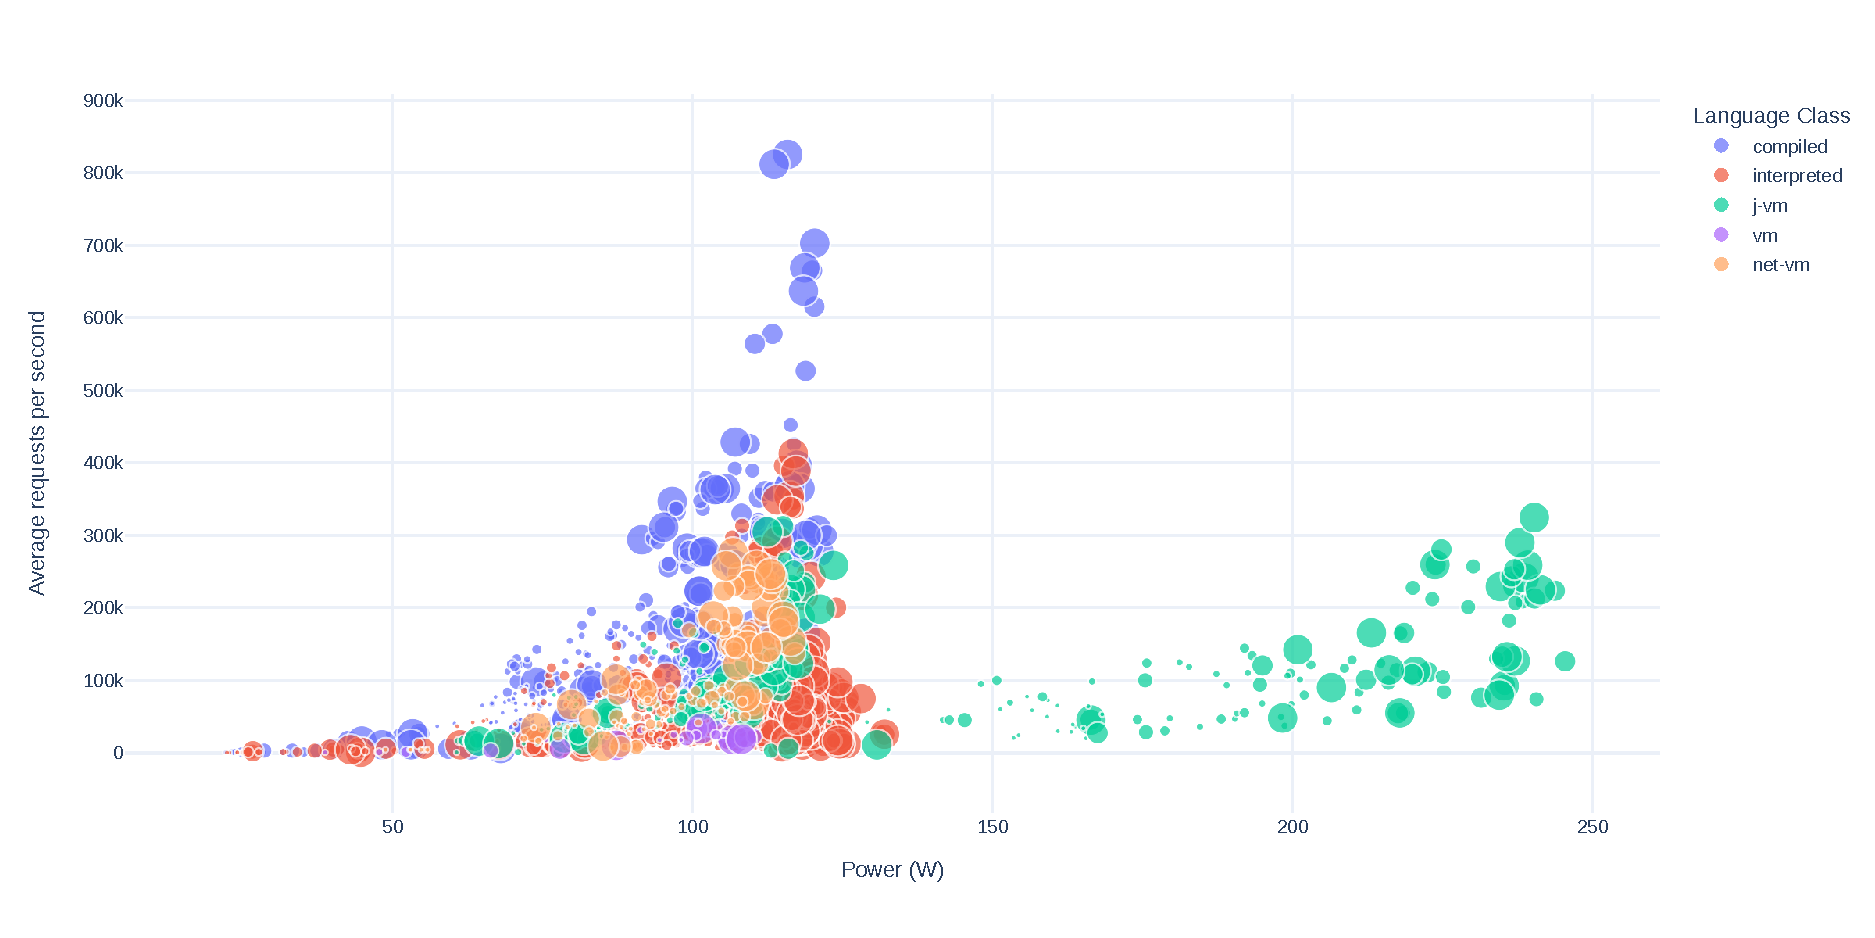
\includegraphics[height=\textwidth,width=\textheight,keepaspectratio,angle=90]{imgs/power_requests_db}
    \caption{Total request vs. average power consumption for the \emph{single query} scenario (size of circles represents the number of clients)}
    \label{fig:power_requests_db}
\end{figure}

\paragraph{Multiple queries}
\begin{figure}[!h]
    \centering
    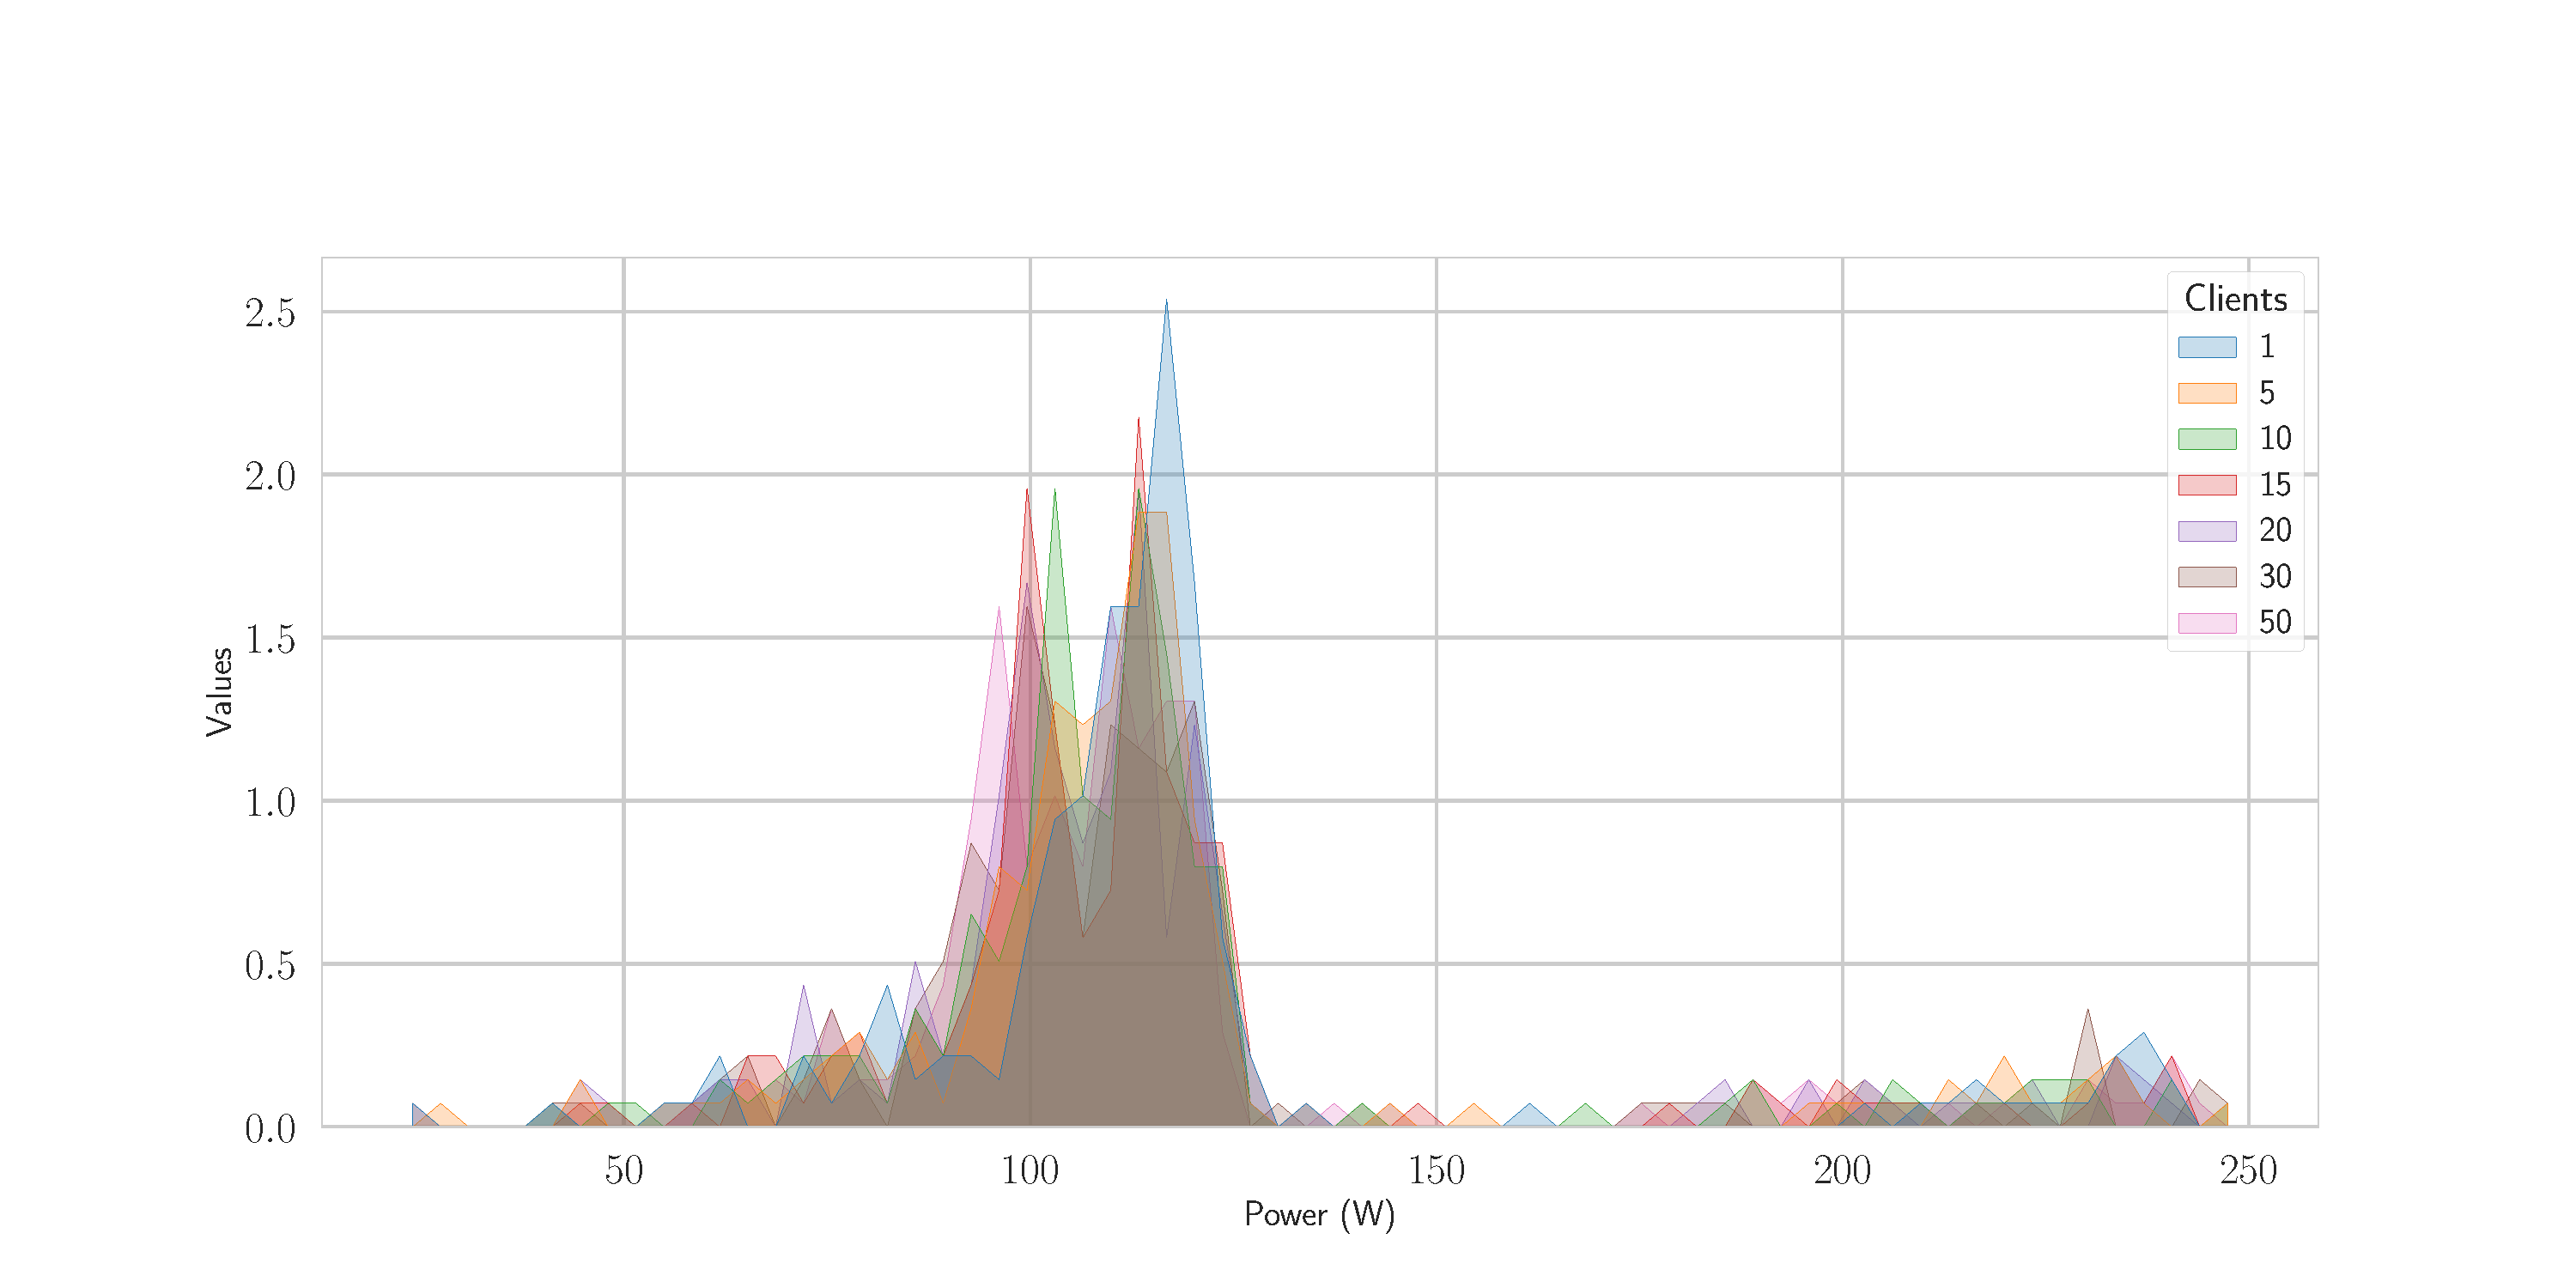
\includegraphics[width=\textwidth,height=\textheight,keepaspectratio]{imgs/histogram_av_power_cpu_query}
    \caption{Distribution of average power consumption for the \emph{multiple queries} scenario }
    \label{fig:av_power_query}
\end{figure}

This scenario benchmarks the framework's efficiency in handling multiple-row queries.
As mentioned before, this study focuses on a fixed number of concurrent clients while we increase the request size per level.

Figure~\ref{fig:av_power_query} reports on the distribution average power consumption for each level.
As one can notice, the query size has no substantial impact on the average power consumption.
Furthermore, one can notice a slight decrease in the average power consumption (from 110 watts to 90 watts) when the size is more significant than ten rows.
This unexpected behavior might be related to the time the database takes to process the query; therefore, the client is resting while waiting for the database answer.
Therefore, one can conclude that the query size has more impact on the database than the framework itself.
To verify this hypothesis, we compare the average power consumption of the database by combining all the frameworks for each database.
Table~\ref{table:query_db_row} details the average power consumption per level for each database.
One can see that for MySQL, there were no changes regardless of the query size, while for Postgres and MongoDB, there is a slight decrease in the average power consumption when the query size is more significant than ten rows. Therefore we can conclude that the type of database had more impact on the average power consumption than the size of the request.


\begin{table*}[!h]
    \raggedright
    \caption{Average power consumption of frameworks based on the database type}
    \label{table:query_db_row}
    \resizebox{\textwidth}{!}{
        \begin{tabular}{l|c|c|c|c|c|c|c|}
            \toprule
            \textbf{Query size} & 1      & 5      & 10     & 15     & 20     & 30     & 50     \\
            \hline
            MongoDB             & 97.17  & 96.93  & 93.38  & 92.58  & 91.61  & 92.585 & 91.17  \\
            MySQL               & 113.86 & 112.92 & 112.74 & 113.05 & 112.13 & 112.62 & 112.16 \\
            PostgresSQL         & 113.86 & 108.25 & 106.19 & 102.97 & 103.41 & 101.95 & 102.96 \\
            \bottomrule
        \end{tabular}}
\end{table*}


\begin{figure}[!h]
    % \centering
    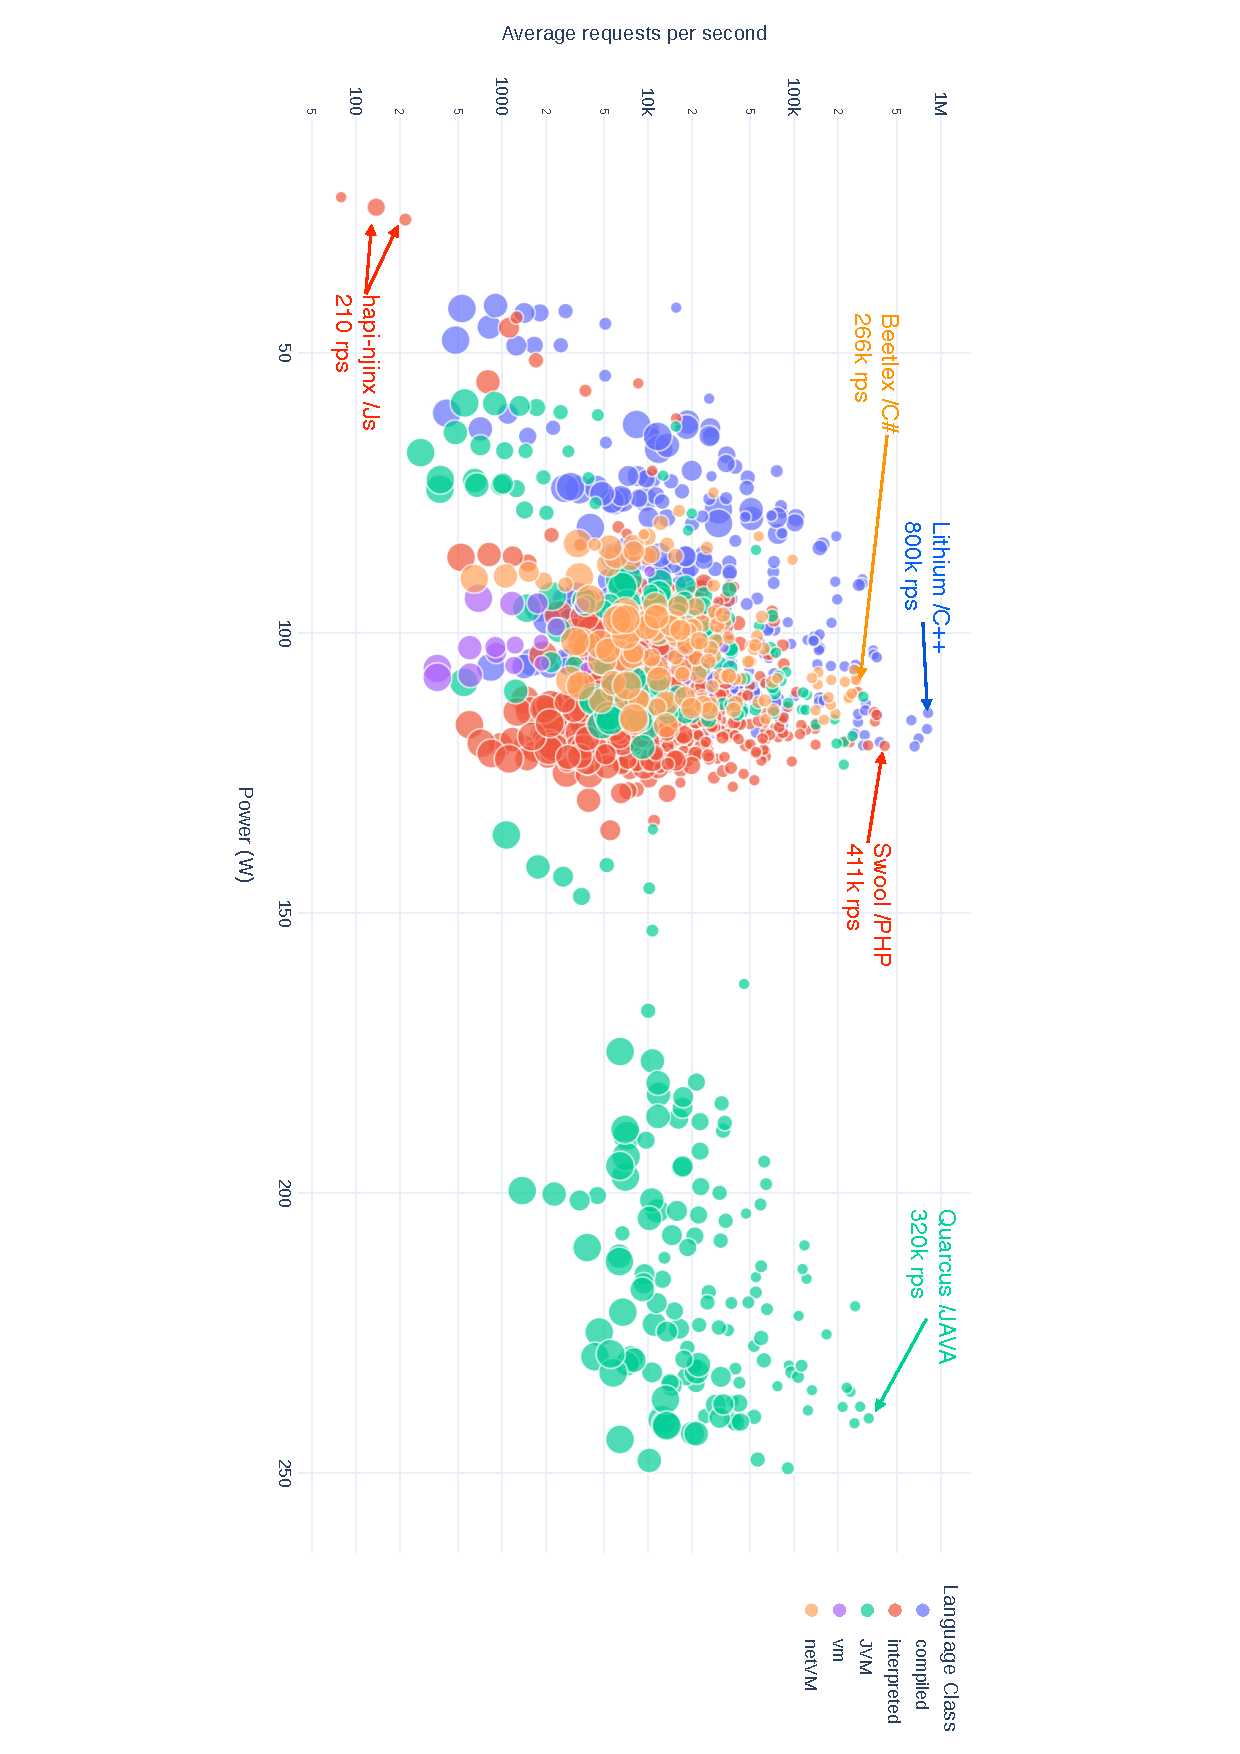
\includegraphics[height=\textwidth,width=\textheight,keepaspectratio,angle=90]{imgs/power_requests_query_log}
    \caption{Total request vs. average power consumption for \emph{multiple queries} scenario (size of circles represents the number of clients)}
    \label{fig:power_requests_query}
\end{figure}

After looking at the power distribution within the multiple query scenario, we will analyze each family separately.

We consider the number of requests per second (aka RPS) as a related performance metric.
Figure~\ref{fig:power_requests_query} presents the total RPS per level for each framework on a logarithmic scale due to the significant performance scale between multiple frameworks.
As one can notice, the difference between the best performing framework, aka Lithium,\footnote{\url{https://matt-42.github.io/lithium/}} and the worst one, aka Hapi-Nginx,\footnote{\url{https://github.com/hapijs/hapi}} is $4,000$ times. At the same time, the average power consumption is five times (120 for lithium vs. 25 for Hapi).This highlight the importance of the clients' number when choosing the framework.

Moreover, one can notice that Java-based frameworks tend to consume more power compared to other languages, with a slight increase in performance.

Finally, PHP remains one of the most efficient frameworks in terms of performance while keeping low average power consumption.



\paragraph{Update}

This scenario tests the framework's efficiency in handling update queries.
As mentioned before, for this study, we will focus on the fixed number of parallel clients while increasing the request size per each level.
Figure~\ref{fig:av_power_update} presents the distribution of average power consumption for each level.
As one can notice, the query size does not strongly impact the average power consumption.
Moreover, the overall average power consumption decreased by 20 Watts. This decrease might be again related to the database processing time.

\begin{figure}[!h]
    \centering
    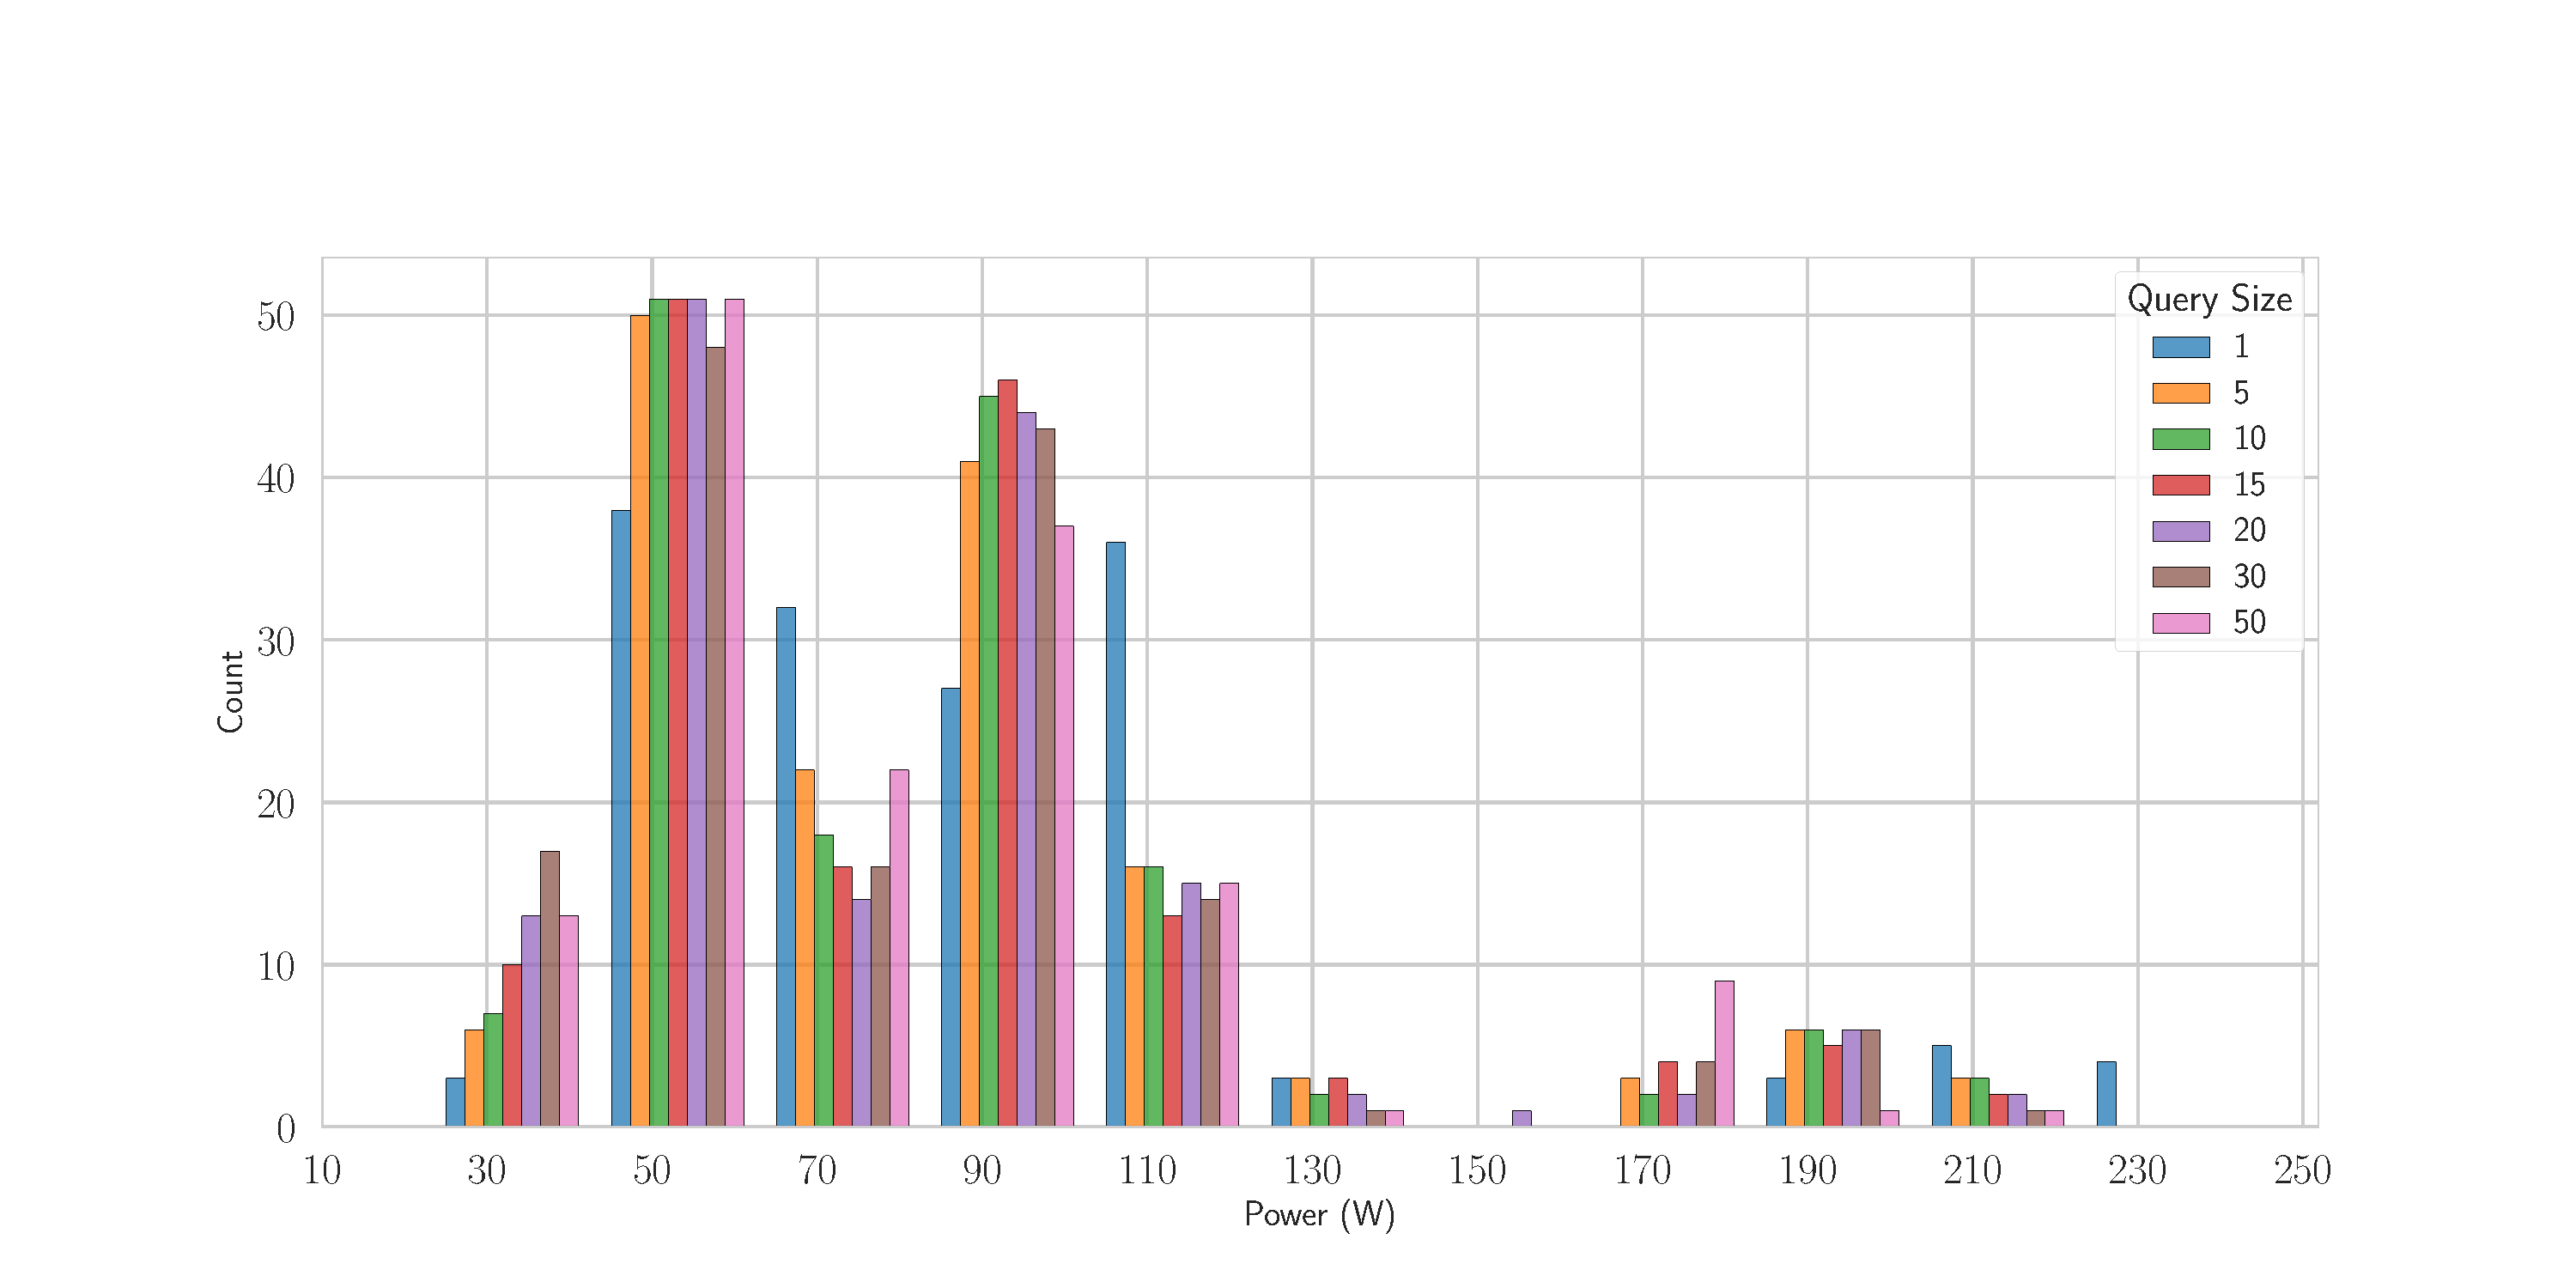
\includegraphics[width=\textwidth,height=\textheight,keepaspectratio]{imgs/histogram_av_power_cpu_update}
    \caption{Distribution of the average power consumption for the \emph{update} scenario}
    \label{fig:av_power_update}
\end{figure}

\begin{figure}[!h]
    % \centering
    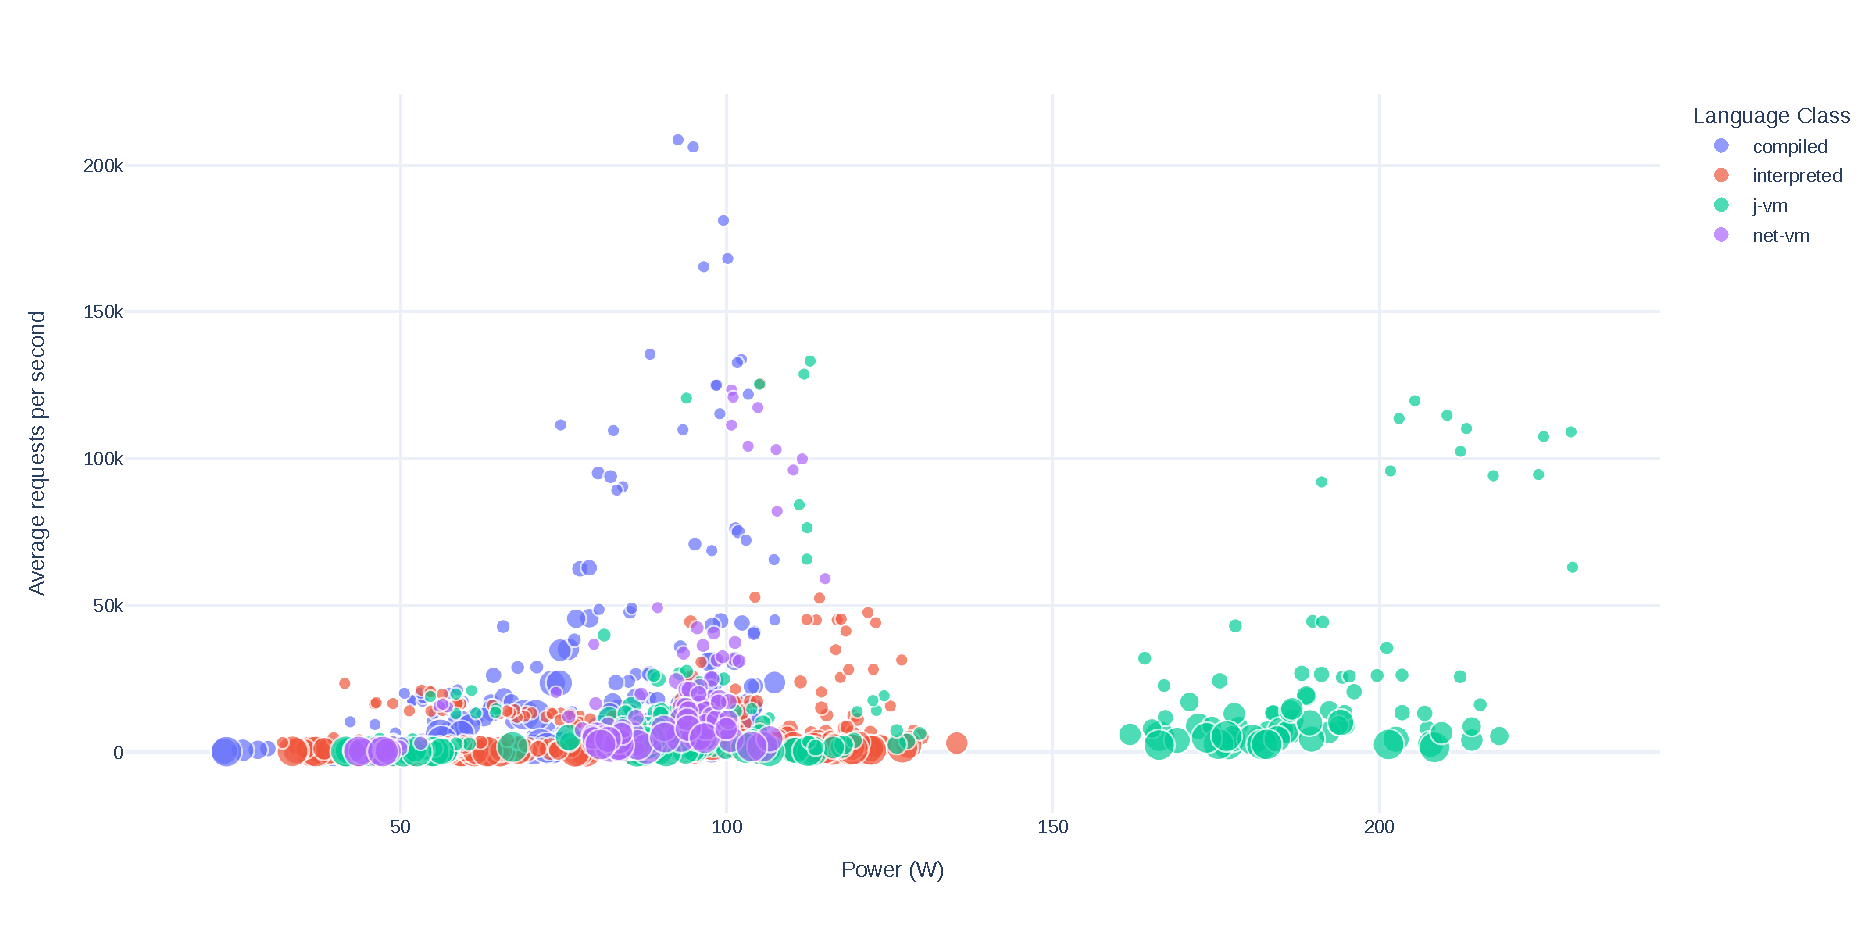
\includegraphics[height=\textwidth,width=\textheight,keepaspectratio,angle=90]{imgs/power_requests_update}
    \caption{Total request vs. average power consumption for the \emph{Update} scenario (size of circles represents the number of clients)}
    \label{fig:power_requests_update}
\end{figure}
Figure~\ref{fig:power_requests_update} reports on the number of RPS per level for each framework.
Swoole dropped in terms of performance while reducing the average power, unlike compiled languages-based frameworks, such as lithium and actise.net, which kept the same performance ranking and average power consumption.
Another interesting observation is that for the compiled languages, both the performance and the average power consumption decrease when the size of the requests increase.
This drop comes with a slight decrease in average power.

\paragraph{Fortunes}
\begin{figure}[!h]
    \centering
    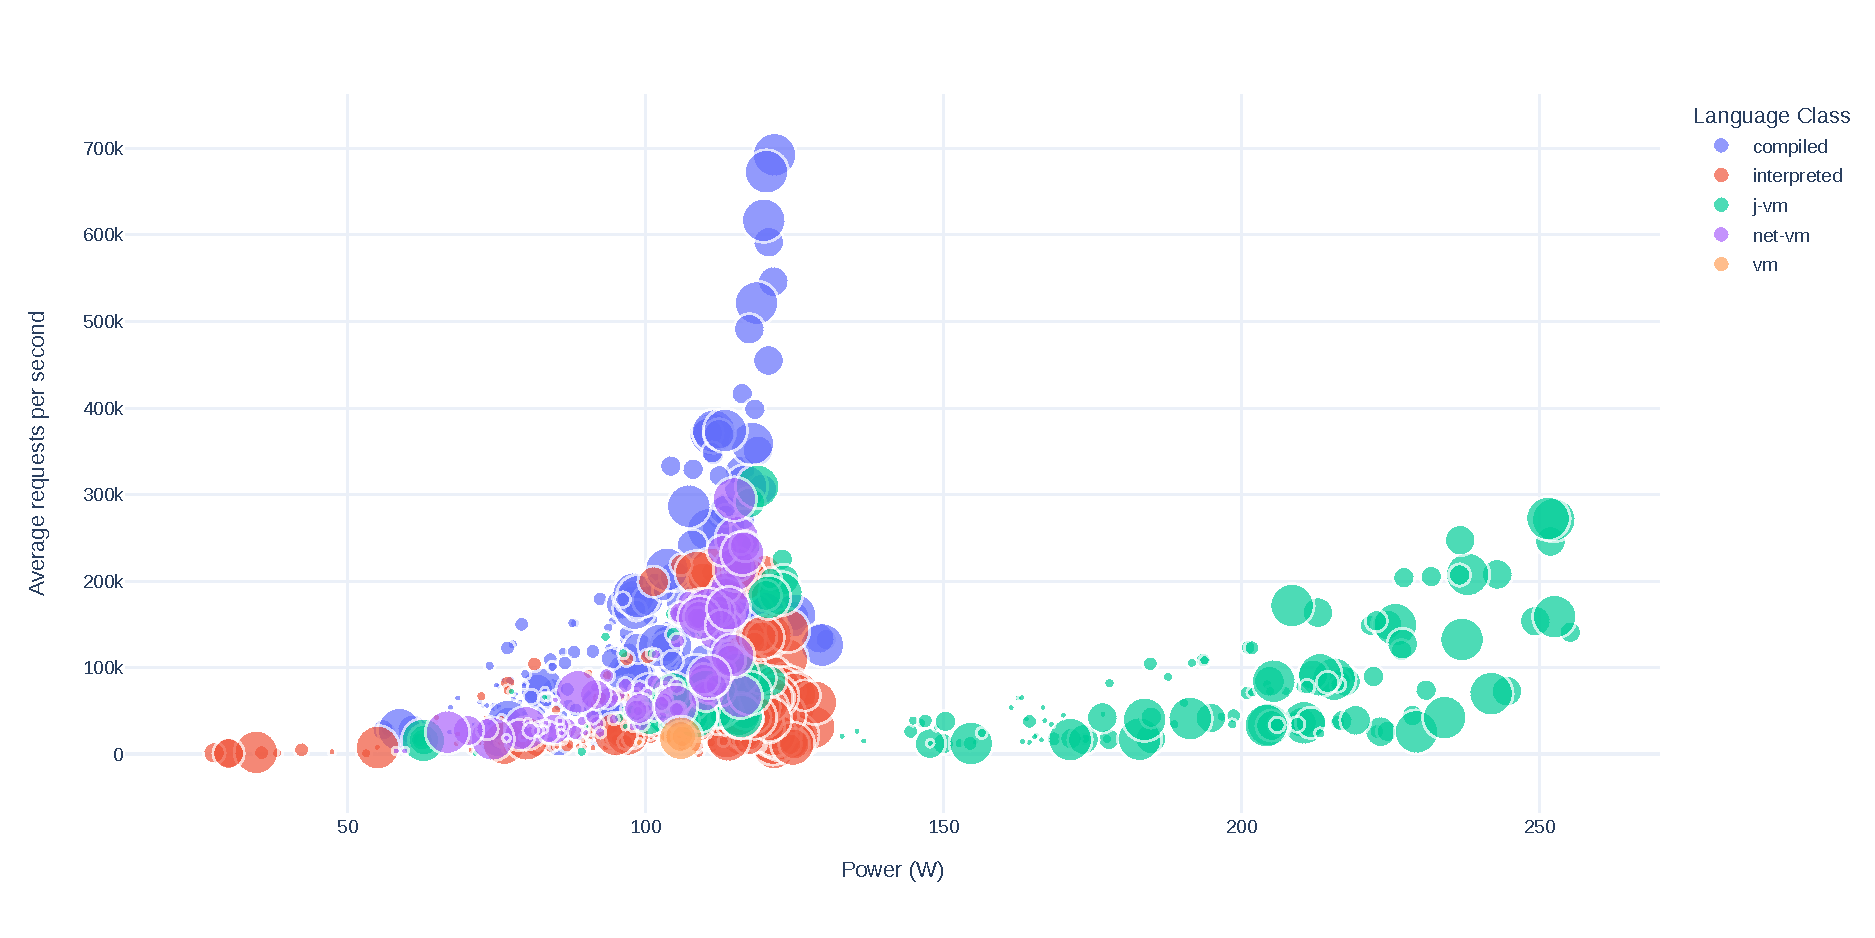
\includegraphics[width=\textwidth,height=\textheight,keepaspectratio]{imgs/power_requests_fortune}
    \caption{Total request vs. average power consumption for \emph{Fortunes}  scenario (size of circles represents the number of clients)}
    \label{fig:power_requests_fortunes}
\end{figure}
The primary purpose of this test is to show the behavior of frameworks when rendering webpages with dynamic content.
As one can see in Figure~\ref{fig:power_requests_fortunes}, Unlike the \emph{single query} scenario. the more clients are connected, the more the performance performances increase. Moreover, we notice a drop in the performance of all interpreted languages, including PHP, that exceeded many compiled frameworks in the other scenarios.

\paragraph{Plain Text and JSON Serialization}
Unforntantly, In these scenario, the client hits its limit before servers, as highlighted in Figures~\ref{fig:power_requests_plaintext},\ref{fig:power_requests_json}.
The ceiling is almost linear for the compiled frameworks and the JVM-based ones.
This is also explained by the fact that, unlike in other scenarios, the high-stress level is on top.
\begin{figure}[!h]
    \centering
    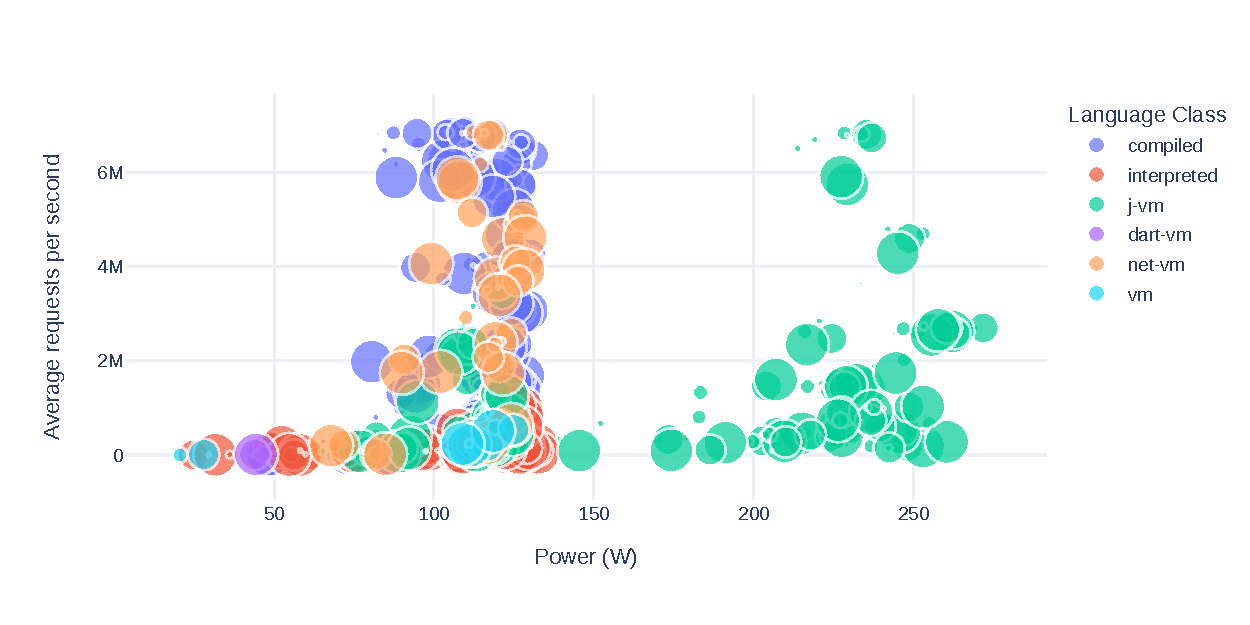
\includegraphics[width=\textwidth,height=\textheight,keepaspectratio]{imgs/power_requests_plaintext}
    \caption{Total request vs. average power consumption for \emph{plainText} scenario (size of circles represents the number of clients)}
    \label{fig:power_requests_plaintext}
\end{figure}

\begin{figure}[!h]
    \centering
    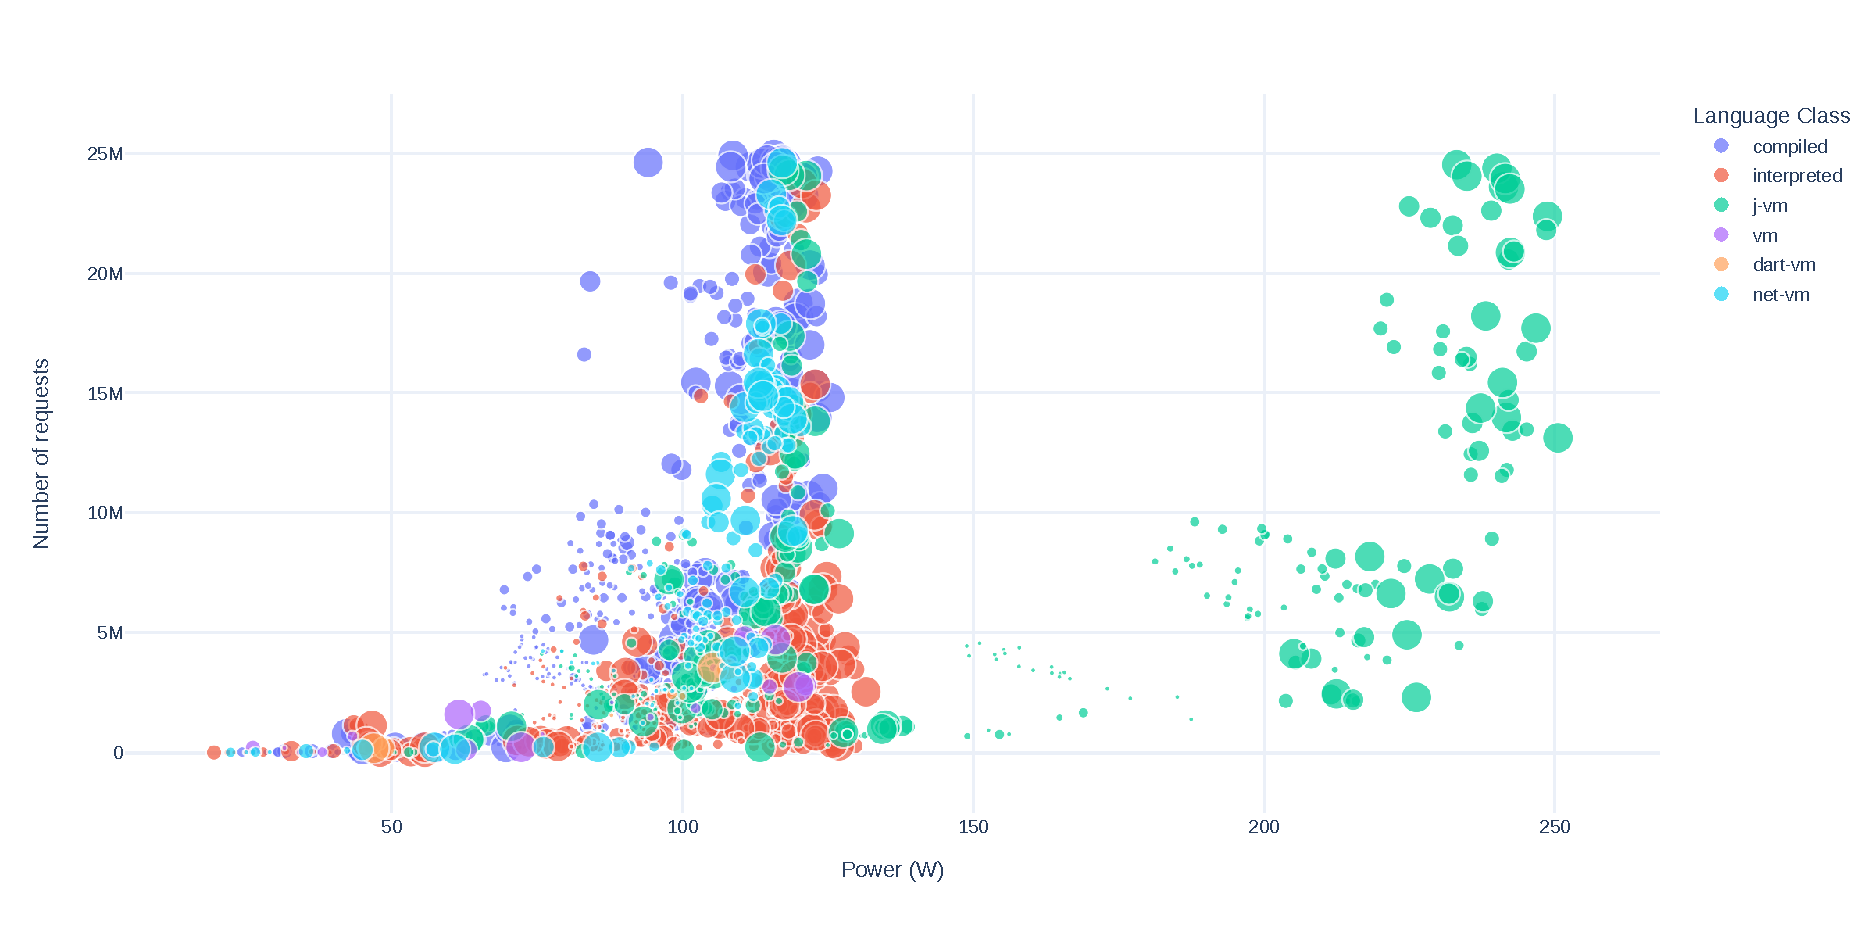
\includegraphics[width=\textwidth,height=\textheight,keepaspectratio]{imgs/power_requests_json}
    \caption{total request vs. average power consumption for \emph{JSON Serialization} scenario (size of circles represents the number of clients)}
    \label{fig:power_requests_json}
\end{figure}

\subsection{Tools}\label{sec:tools}
\textsf{GreenBoard}\url{https://github.com/chakib-belgaid/greenboard} is an open-source dashboard designed to assist developers and practitioners in selecting the most energy-efficient web framework based on their requirements.
It enables the user to compare the performance and energy consumption of different frameworks. As well as filtering the frameworks based on their programming language, the database type, and other criteria.
This dashboard is designed based on the latest results obtained from our experiments and we will keep updating it with the latest results.
\cref*{fig:raw_table_example} presents an example of the raw obtained after selecting 7 frameworks. For the sake of versatility, we will consider the \emph{single query} scenario with two levels of clients (64 and 256).
As one can see, although \textsf{Spark} depicts the highest amount of powers (235W), it is ranked 6th when it comes to the energy consumed per request. On the other hand, \textsf{Flask-pypy} consumed half of its power (118W) but it pays in terms of performance with ten times slower latency, and its requests cost seven times more than \textsf{Spark's} requests.
In terms of performance and energy consumption, PHP, on the other hand, contained both, the best and the worst frameworks. Therefore one should be careful when choosing a framework and its configurations rather than just the language.

\begin{figure}[!h]
    \centering
    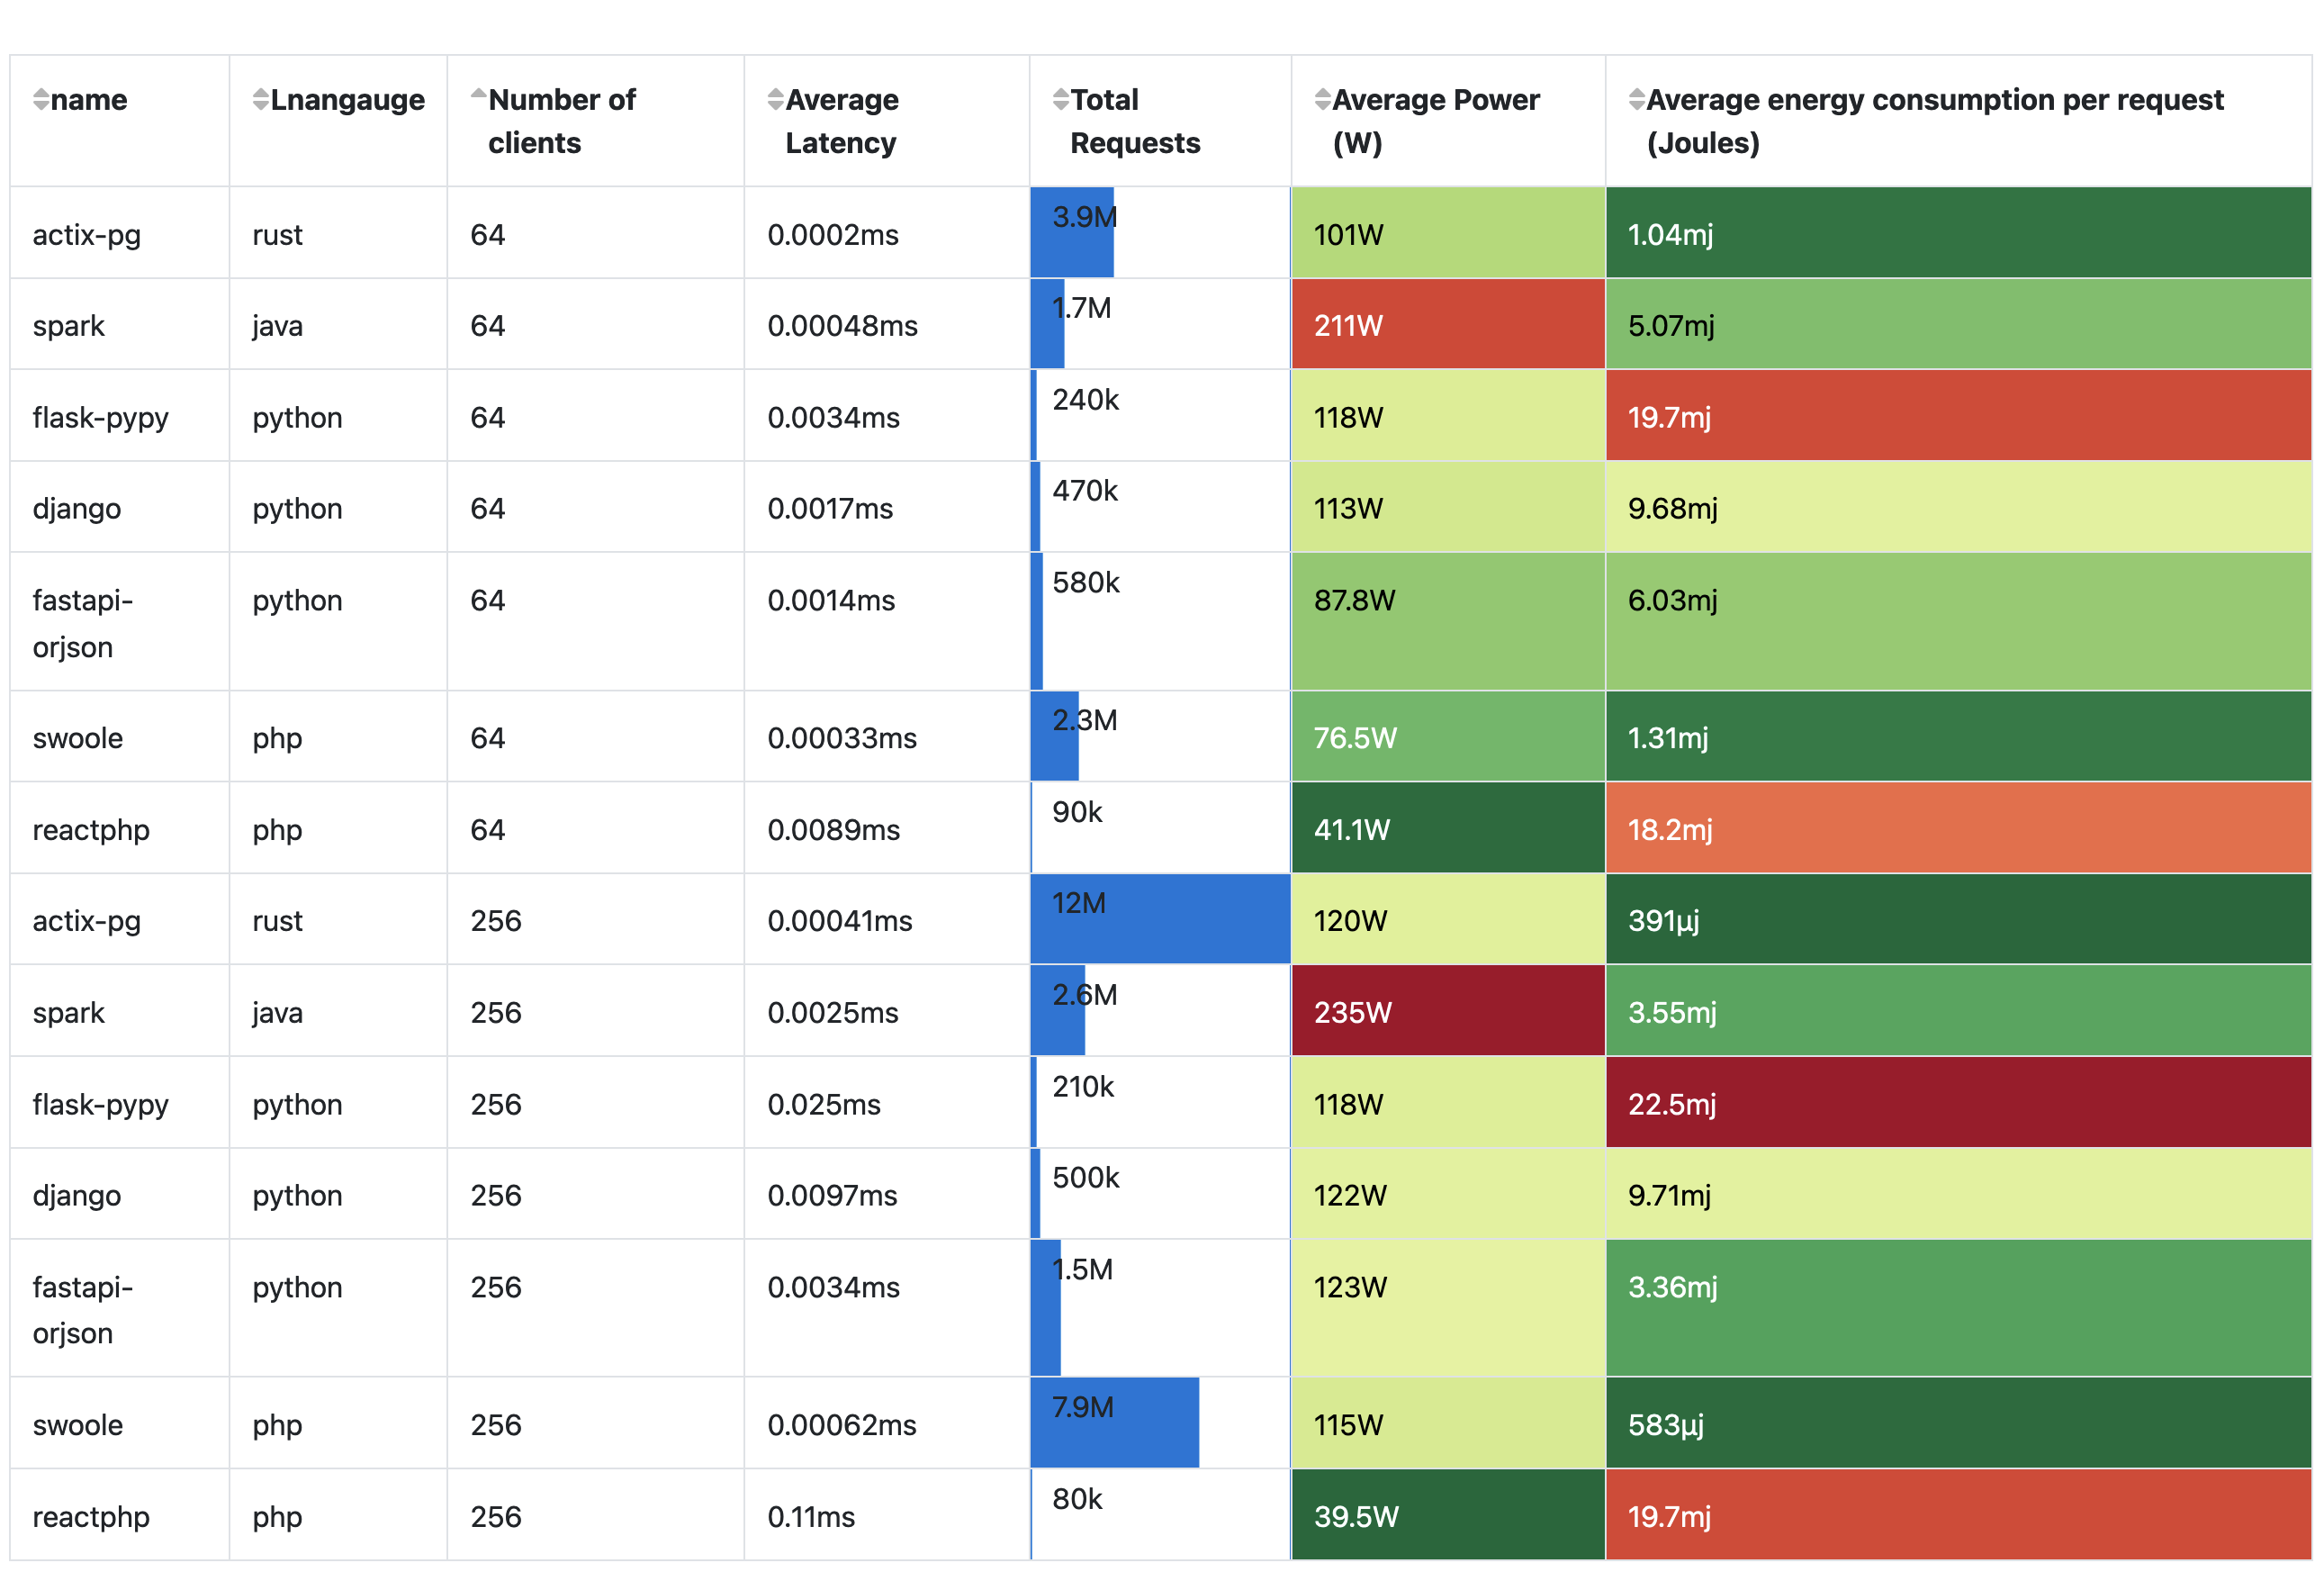
\includegraphics[width=\textwidth,height=\textheight,keepaspectratio]{example/thesis_exp_raw_table}
    \caption{Example of measurement for the \emph{single query} scenario}
    \label{fig:raw_table_example}
\end{figure}


\subsection{Summary}
\begin{figure}[!h]
    \centering
    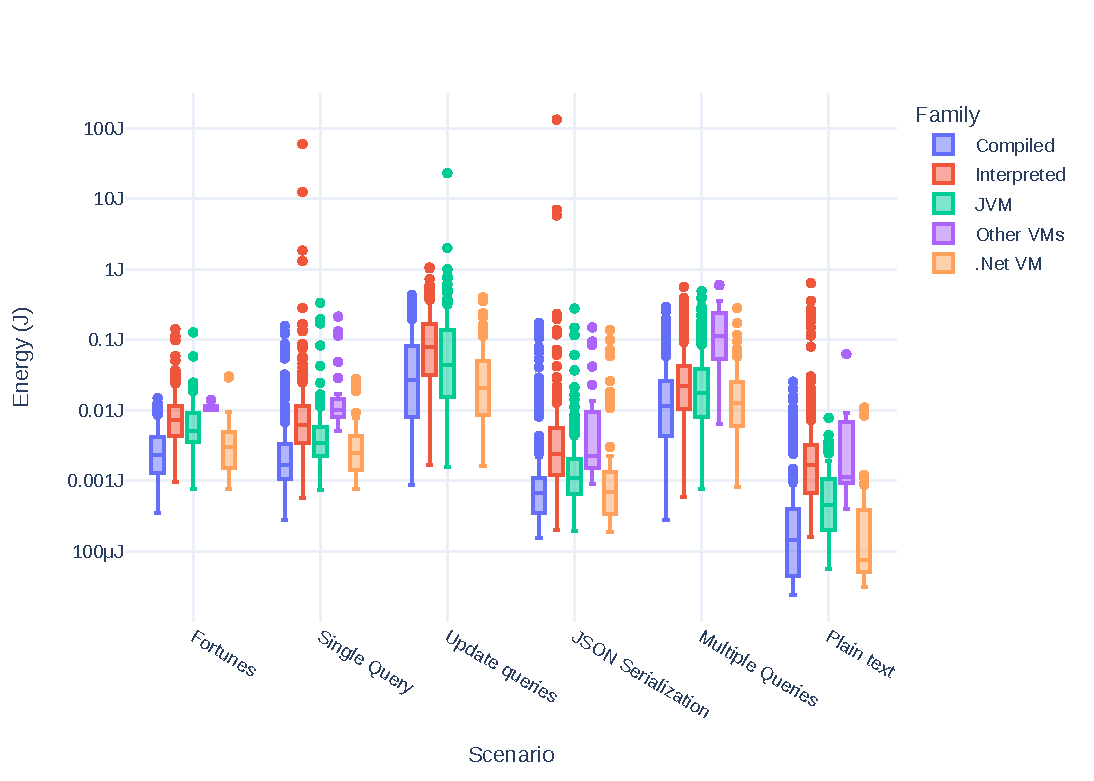
\includegraphics[width=.9\columnwidth ]{imgs/all_boxplot}
    \caption{Energy consumption per request for each family of programming languages}
    \label{fig:all_boxplot}
\end{figure}

This section presents a study on several web frameworks' performance and power consumption.
To do so, we used the \emph{TechEmpower}\footnote{\url{https://www.techempower.com/benchmarks}} benchmark suite, which is a set of tests that measure the performance of several web frameworks.
We tested $261$ frameworks using $7$ scenarios.
We found that Java-based frameworks are the most power-consuming, while the complied ones are the most efficient in terms of performance.
Moreover, PHP remains one of the most efficient frameworks in terms of performance and energy despite being an interpreted language.
This behavior is mainly due to the optimization done on the Zend engine\footnote{\url{https://www.zend.com/}} to fit the website's requirements.
Furthermore, we found that the database impacts the energy consumption and the average power of the servers even when they are not on the same machine.
To summarize our findings, we present in \cref{fig:all_boxplot} a comparison of the energy consumption per request for each scenario.
While we have seen in the previous results that Java-based frameworks depict the highest energy; they still provide greener requests compared to the interpreted frameworks; this is mainly because their interpreters report lower performances.


% \begin{figure}[bht]
%     \centering
%     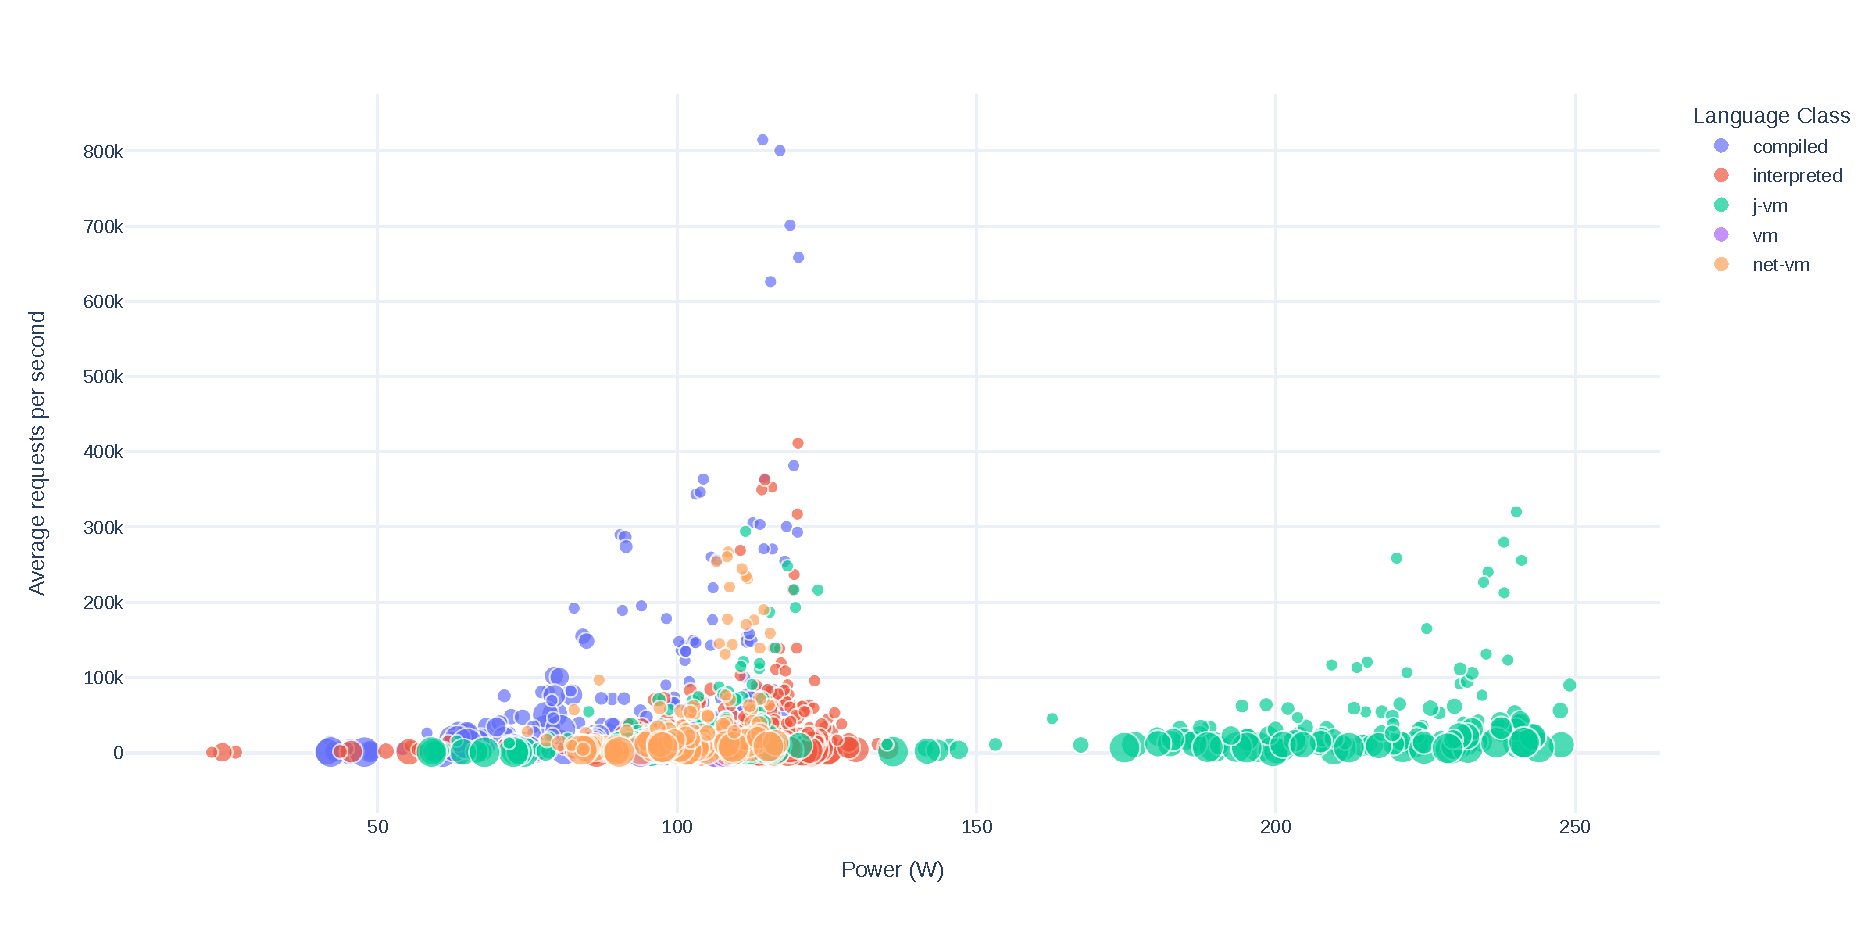
\includegraphics[width=
%         \columnwidth]{imgs/power_requests_query}
%     \caption{total request vs average power consumption for the multiple queries test ( Size of circles represents the size of the query )}
%     \label{fig:power_requests_query}
% \end{figure}
% \begin{figure}[bht]
%     \centering
%     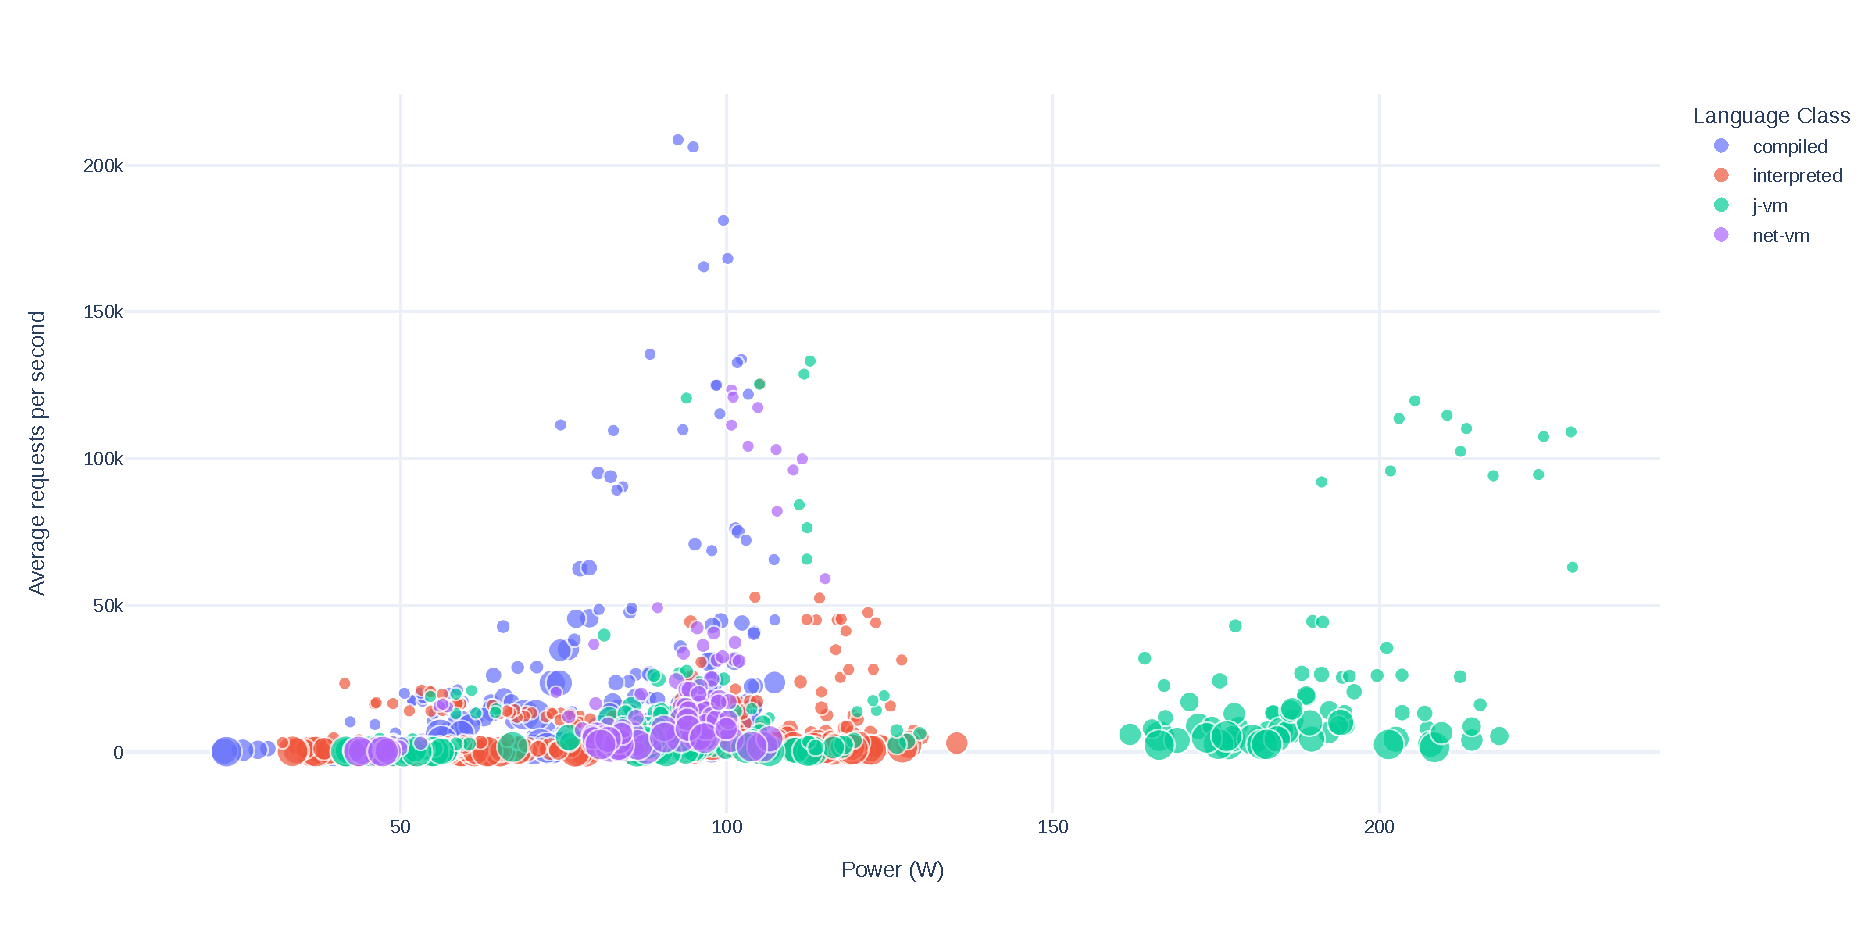
\includegraphics[width=
%         \columnwidth]{imgs/power_requests_update}
%     \caption{total request vs average power consumption for the update queries test ( Size of circles represents the size of the query )}
%     \label{fig:power_requests_update}
% \end{figure}
% \begin{figure}[bht]
%     \centering
%     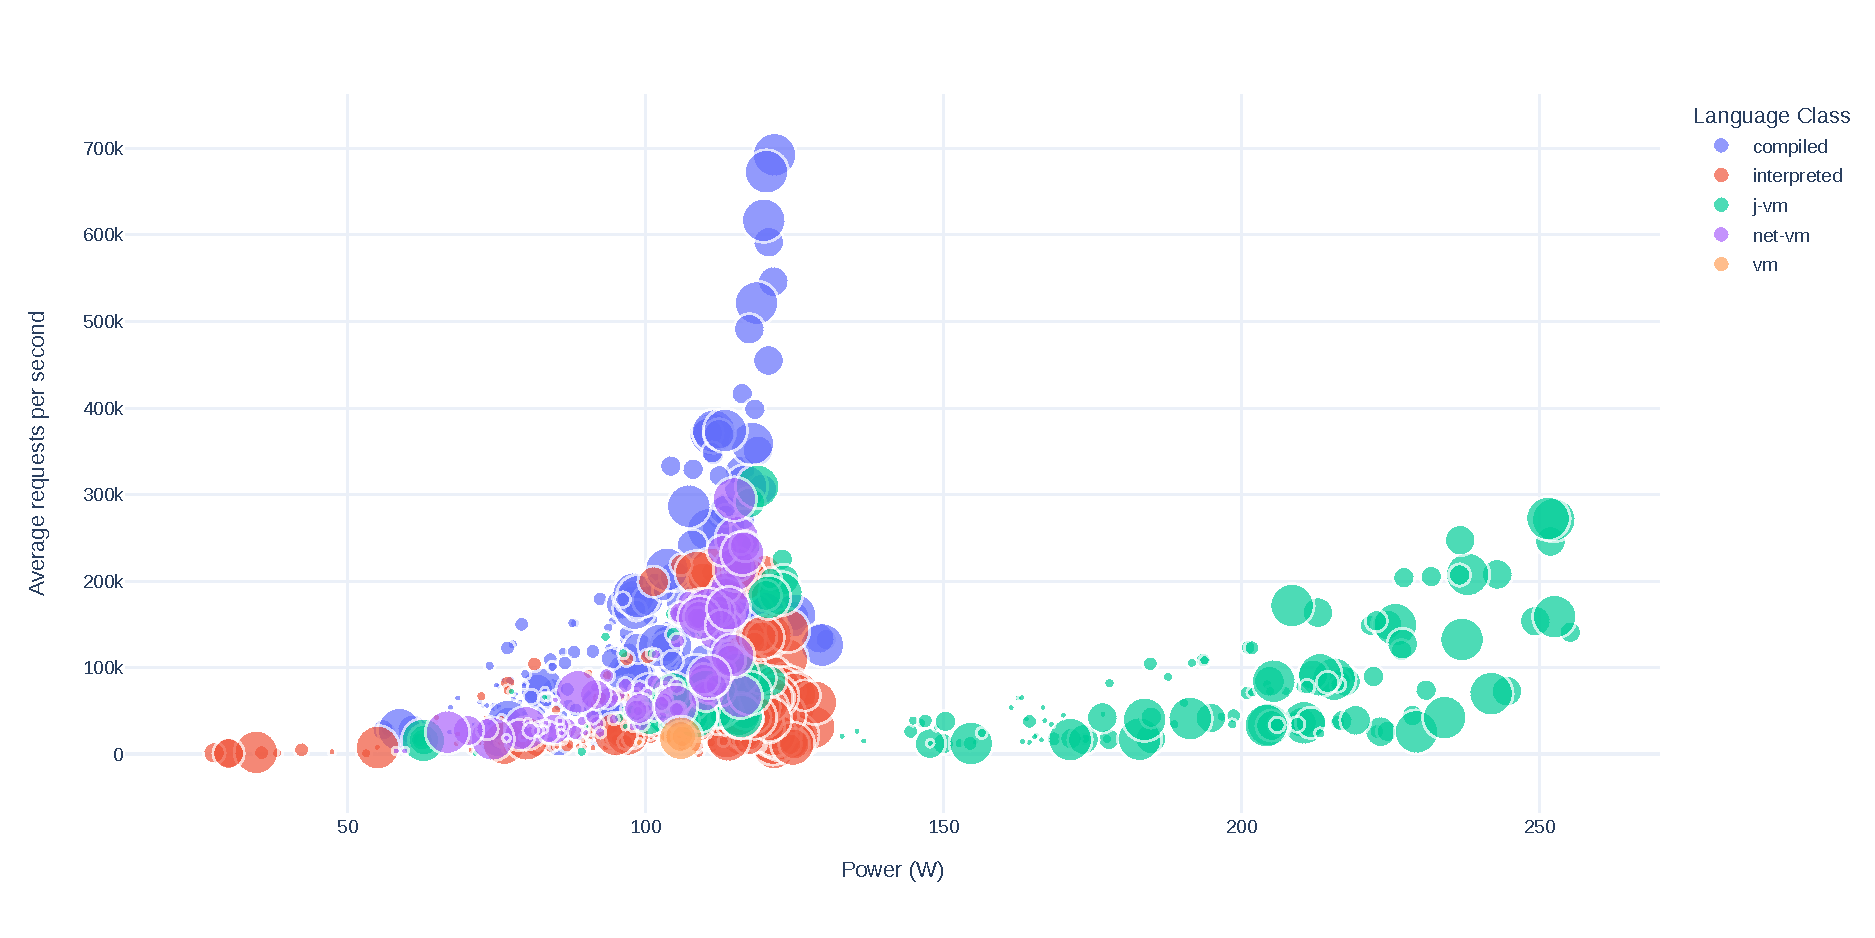
\includegraphics[width=
%         \columnwidth]{imgs/power_requests_fortune}
%     \caption{total request vs average power consumption for Fortunes test ( Size of circles represents the number of clients)}
%     \label{fig:power_requests_fortune}
% \end{figure}
% \begin{figure}[bht]
%     \centering
%     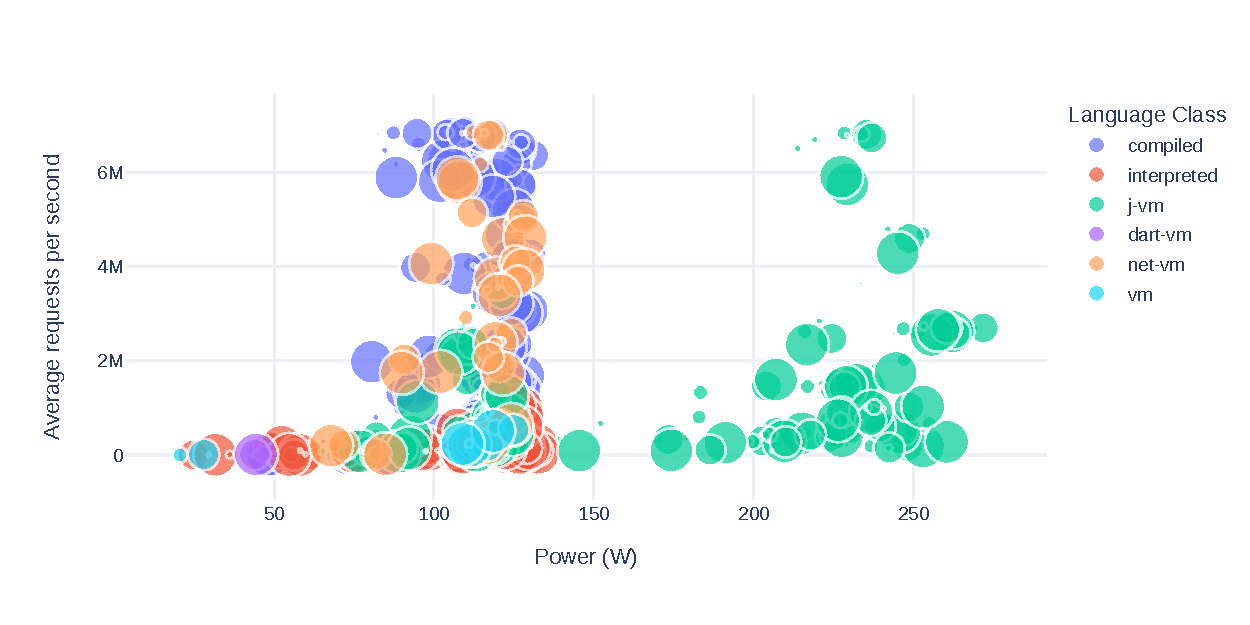
\includegraphics[width=
%         \columnwidth]{imgs/power_requests_plaintext}
%     \caption{total request vs average power consumption for plainText test (size of circles represents the number of clients)}
%     \label{fig:power_requests_plaintext}
% \end{figure}
% \begin{figure}[bht]
%     \centering
%     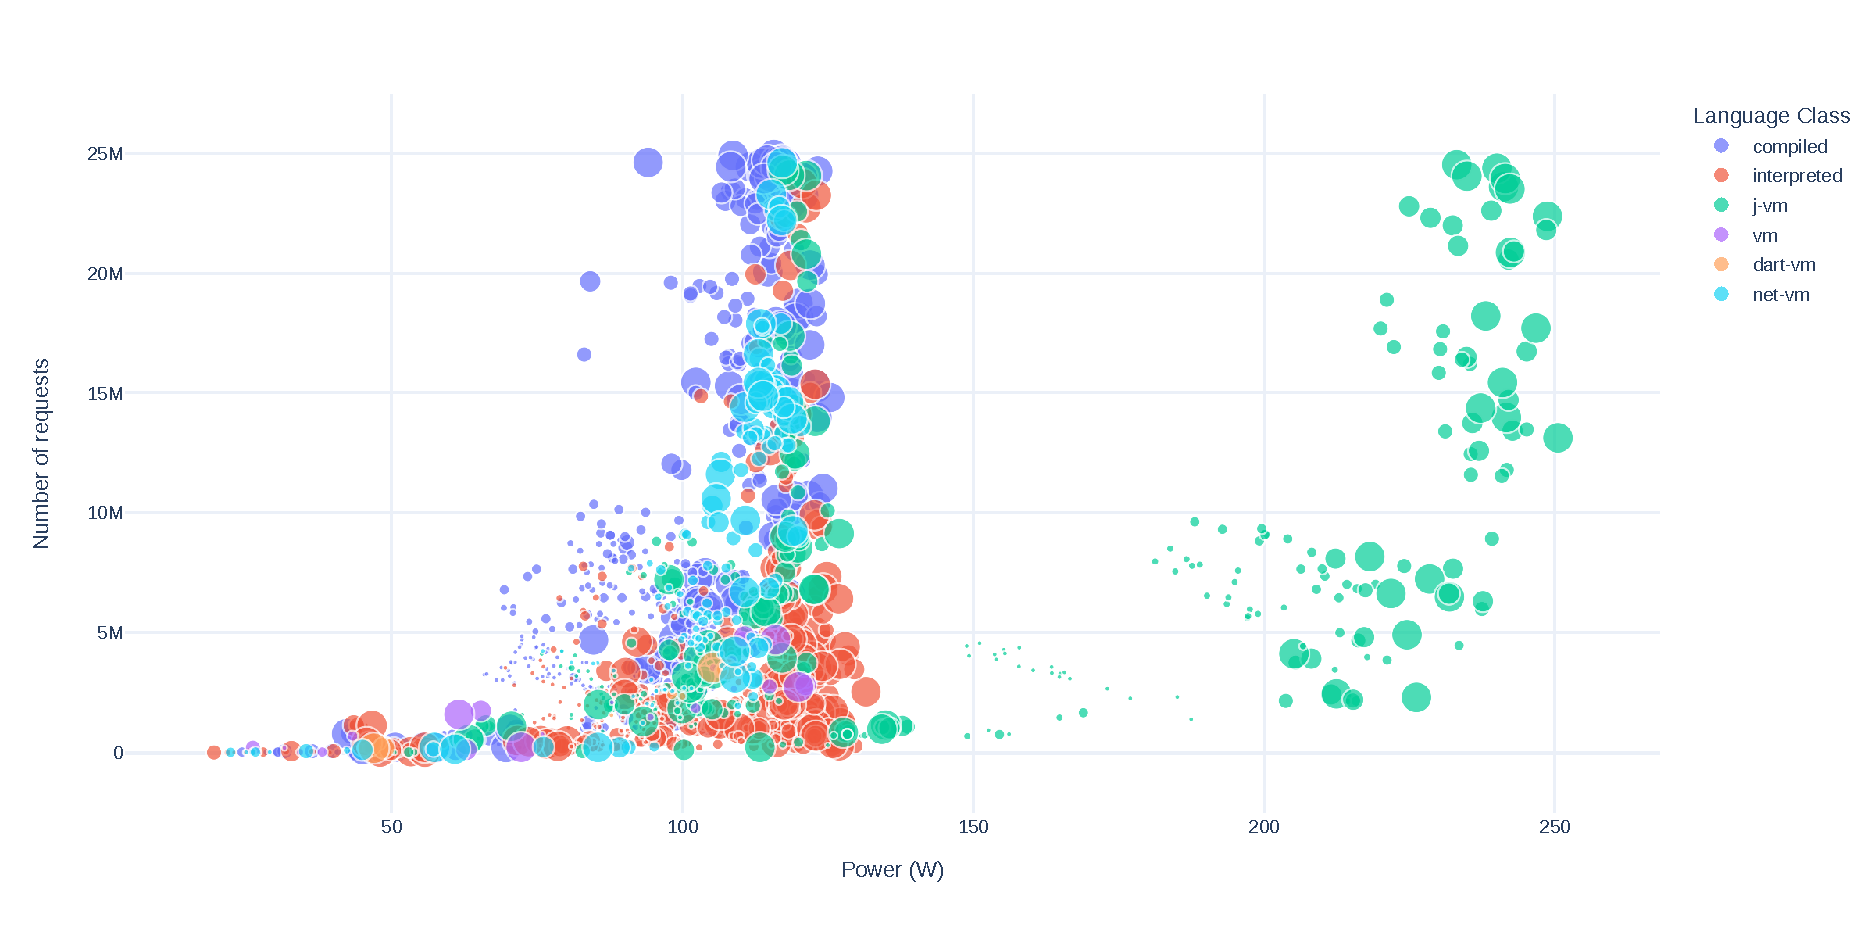
\includegraphics[width=
%         \columnwidth]{imgs/power_requests_json}
%     \caption{total request vs average power consumption for JSON Serialization test (size of circles represents the number of clients)}
%     \label{fig:power_requests_json}
% \end{figure}
% to reduce the space of research we will be looking for some correlation 
% same thing for the number of clients, maybe we gonna consider 3 cases - 0, low and high 

%  when comparing static vs dynamic programming languages we exclude the ones that use reflection aka C# and JAVA

%% for more about the syntax we recommend checking this website https://learnxinyminutes.com/

% \newpage

% \subsubsection{tools}
